\documentclass[11pt,a4paper]{article}
\usepackage[margin=2.4cm]{geometry}
\usepackage[T1]{fontenc}
\usepackage{lmodern,microtype}
\usepackage{amsmath,amssymb}
\usepackage{siunitx}
\usepackage{booktabs,tabularx,array}
\usepackage{graphicx,xcolor}
\usepackage{caption,subcaption}
\usepackage{enumitem}
\usepackage[section]{placeins}
\usepackage{tikz,pgfplots}
\usetikzlibrary{arrows.meta,decorations.markings,calc}
\pgfplotsset{compat=1.17}
\usepackage{fancyhdr}
\usepackage{titlesec}
\usepackage[hidelinks]{hyperref}
\pagestyle{fancy}\fancyhf{}
\fancyhead[L]{\small\scshape sCO\textsubscript{2} Brayton cycle for a 100\,MWth SMR}
\fancyhead[R]{\small\scshape ME 306, Autumn 2026}
\fancyfoot[C]{\small\thepage}
\renewcommand{\headrulewidth}{0.4pt}
\fancypagestyle{plain}{\fancyhf{}\fancyfoot[C]{\small\thepage}\renewcommand{\headrulewidth}{0pt}}
\titleformat{\section}{\Large\bfseries}{\thesection}{0.8em}{}[\vspace{0.15em}{\color{black!50}\titlerule[0.5pt]}]
\titleformat{\subsection}{\large\bfseries}{\thesubsection}{0.7em}{}
\titlespacing*{\section}{0pt}{1.6em}{1.0em}
\titlespacing*{\subsection}{0pt}{1.2em}{0.5em}
\setlength{\parskip}{0.35em}
\newcommand{\code}[1]{\par\smallskip\noindent{\footnotesize\textbf{Code}\ \textbar\ #1}\par}
\sisetup{detect-all,per-mode=symbol}
\setlist{nosep}
\captionsetup{font=small,labelfont=bf}

\newcommand{\todo}[1]{\textcolor{red}{[TO DO: #1]}}
\newcommand{\scotwo}{sCO\textsubscript{2}}
\newcommand{\cotwo}{CO\textsubscript{2}}
\newcommand{\Ph}{P_\mathrm{high}}
\newcommand{\Pl}{P_\mathrm{low}}
\newcommand{\Pm}{P_\mathrm{mid}}
\newcommand{\Pe}{P_\mathrm{exh}}
\newcommand{\Tin}{T_\mathrm{in}}
\newcommand{\Tt}{T_\mathrm{turb}}

% Shared drawing styles for the cycle block diagrams.
% Every diagram is a loop: high-pressure line on top, low-pressure line below.
\tikzset{
  fl/.style={line width=0.6pt, postaction={decorate},
     decoration={markings, mark=at position 0.55 with {\arrow{Latex[length=5pt]}}}},
  ln/.style={line width=0.6pt},
  box/.style={draw, fill=white, minimum width=11mm, minimum height=6mm, font=\scriptsize, inner sep=2pt},
  hx/.style={draw, fill=gray!12, font=\scriptsize, inner sep=2pt},
  st/.style={font=\scriptsize\itshape, text=black!70, inner sep=1pt},
  nm/.style={font=\scriptsize},
  dot/.style={circle, fill=black, inner sep=1.1pt},
  % compressor: wide inlet on the left, narrow outlet on the right
  pics/comp/.style={code={\draw[fill=white, line width=0.6pt]
     (-0.35,-0.42)--(0.35,-0.22)--(0.35,0.22)--(-0.35,0.42)--cycle;}},
  % turbine: narrow inlet on the left, wide outlet on the right
  pics/turb/.style={code={\draw[fill=white, line width=0.6pt]
     (-0.35,-0.22)--(0.35,-0.42)--(0.35,0.42)--(-0.35,0.22)--cycle;}},
}


\begin{document}

%------------------------------- title page ----------------------------------
\begin{titlepage}
\thispagestyle{empty}
\newgeometry{margin=2.2cm,top=2.4cm,bottom=2.2cm}
\centering
{\large\scshape ME 306 \textbullet{} Applied Thermodynamics\par}
\vspace{0.15cm}
{\small Department of Mechanical Engineering, Indian Institute of Technology Bombay\par}
\vspace{1.1cm}
{\color{black!70}\rule{\textwidth}{0.4pt}}\par\vspace{-0.25cm}
\rule{\textwidth}{1.6pt}\par\vspace{0.55cm}
{\fontsize{22}{27}\selectfont\bfseries Supercritical \cotwo{} Brayton Cycle\\[4pt] for a \SI{100}{MWth} Small Modular Reactor\par}
\vspace{0.4cm}
{\large\itshape Cycle-layout selection under a mass and lifetime-payout trade-off\par}
\vspace{0.5cm}
\rule{\textwidth}{1.6pt}\par\vspace{-0.25cm}
{\color{black!70}\rule{\textwidth}{0.4pt}}\par
\vspace{1.1cm}

\begin{minipage}[t]{0.47\textwidth}\centering
{\small\scshape Team\par}\vspace{0.2cm}
\renewcommand{\arraystretch}{1.3}
\begin{tabular}{@{}l l@{}}
\toprule
Name & Roll number\\
\midrule
Siddhant Patil & 24B2121\\
Vaishnavi Shivai & 24B2116\\
Avinav Shekhar & 24B2186\\
Anshuman Gupta & 24B2169\\
Vidit Ganna & 24B2210\\
\bottomrule
\end{tabular}
\end{minipage}\hfill
\begin{minipage}[t]{0.47\textwidth}\centering
{\small\scshape Course instructor\par}\vspace{0.2cm}
Prof.\ Shankar Krishnan\par
\vspace{0.9cm}
{\small\scshape Project mentor\par}\vspace{0.2cm}
Prof.\ Janani Srree Murallidharan\par
\end{minipage}

\vspace{1.2cm}
\begin{minipage}{0.9\textwidth}
\small
{\centering\scshape Abstract\par}\vspace{0.2cm}
\setlength{\parindent}{0pt}\linespread{1.08}\selectfont
Six supercritical \cotwo{} Brayton cycle layouts are compared for a \SI{100}{MWth} small modular reactor with a turbine inlet limit of \SI{500}{\celsius} and \SI{20}{MPa}: simple, recuperated, recompression, recuperated with intercooling, recompression with intercooling, and partial cooling. Each layout is solved with real-gas properties over a grid of pressures, compressor inlet temperatures and split fractions (1053 designs, 969 feasible). Heat-exchanger conductance is converted to mass, and designs are ranked on mass and on ten-year payout (electricity revenue less hardware cost) by a Pareto front, its knee point and TOPSIS. The simple cycle is reported but left out of the ranking, as it is not a credible candidate. The fixed mass is calibrated so that the best recuperated design (33.3\% efficiency) has the given baseline mass of \SI{60}{t}. The recommended design is the recompression cycle at \SI{20}{MPa}, \SI{7.7}{MPa} and \SI{33}{\celsius} compressor inlet and a split fraction of 0.40. It reaches 40.2\% efficiency at \SI{71.5}{t}, with a ten-year payout (electricity value less hardware cost, a comparative measure only) of \$178.9M against \$148.2M for the recuperated baseline. Its extra output recovers the cost of its extra hardware in about ten months. It gives up 2.1 points of efficiency and 4.7\% of payout against the highest-payout design found (the same cycle at \SI{32}{\celsius} and a split of 0.36), which is \SI{6.7}{t} heavier. Intercooling does not pay in either form.
\end{minipage}

\vfill
{\color{black!70}\rule{0.5\textwidth}{0.4pt}}\par\vspace{0.2cm}
{\small Code and data: \href{https://github.com/scp15156402/SMR_sCO2_Optimiser/tree/rebuild}{\texttt{github.com/scp15156402/SMR\_sCO2\_Optimiser/tree/rebuild}}\par}
\vspace{0.25cm}
{\scshape Autumn 2026\par}
\restoregeometry
\end{titlepage}

%------------------------------- contents ------------------------------------
\setcounter{page}{2}
{\linespread{0.96}\selectfont\tableofcontents}
\newpage

\section{Problem statement}

A small modular reactor (SMR) is built in a factory and shipped in modules, so its power conversion system must be compact. A closed Brayton cycle using supercritical carbon dioxide (\scotwo) is a candidate because \cotwo{} is dense, and near its critical point (\SI{7.38}{MPa}, \SI{30.98}{\celsius}) it needs little work to compress.

The benefit depends on the cycle layout. A simple recuperated cycle is limited by a mismatch in specific heat between the two sides of the recuperator. More complex layouts reduce that mismatch and raise efficiency, but they add heat exchangers and compressors. That extra hardware adds mass and cost, which works against the reason for choosing \scotwo.

This project takes a \SI{100}{MWth} reactor as the heat source and asks: \emph{which cycle layout and operating point should be recommended, when efficiency has to be weighed against the mass and cost of the hardware that delivers it?}

The work has four parts:
\begin{enumerate}
  \item Model six cycle layouts with real-fluid properties.
  \item Sweep each layout over its operating variables, within the given limits.
  \item For every feasible design, compute the thermal efficiency and the conductance ($UA$) of each heat exchanger, and from these the hardware mass, hardware cost and lifetime payout.
  \item Find the designs that are not beaten on both payout and mass (the Pareto front), and select one.
\end{enumerate}

All given numerical values are illustrative classroom figures and not data for a real reactor.

\section{Working fluid: why real-gas properties are needed}

The ideal-gas relations ($Pv = RT$, constant $c_p$) do not hold for \cotwo{} near its critical point. Two property plots show why, and both matter for the cycle.

\paragraph{Compression work is low.} Figure~\ref{fig:z} shows the compressibility factor $Z = Pv/RT$ along the \SI{7.7}{MPa} isobar. An ideal gas has $Z = 1$. At the given minimum compressor inlet state (\SI{32}{\celsius}, \SI{7.7}{MPa}), $Z = 0.22$ and the density is \SI{602}{kg/m^3}, closer to a liquid than a gas. Compressor work is $\int v\,dP$, so a dense fluid takes little work to compress.

For isentropic compression from \SI{7.7}{MPa} to \SI{20}{MPa} starting at \SI{32}{\celsius}:
\begin{center}
\begin{tabular}{lS[table-format=2.1]}
\toprule
Method & {Specific work (\si{kJ/kg})}\\
\midrule
Real-fluid properties (CoolProp) & 18.3\\
Ideal gas, constant $c_p$ ($k = 1.285$) & 61.3\\
\bottomrule
\end{tabular}
\end{center}
The ideal-gas formula overstates the work by a factor of 3.4. A cycle model built on it would be wrong where it matters most.

\paragraph{Specific heat varies strongly.} Figure~\ref{fig:cp} shows $c_p$ on the low-pressure side (\SI{7.7}{MPa}) and the high-pressure side (\SI{20}{MPa}). Near the critical point, $c_p$ at \SI{7.7}{MPa} peaks sharply (about \SI{75}{kJ/kg.K} at \SI{32.9}{\celsius}). Between roughly \SI{60}{\celsius} and \SI{250}{\celsius}, which is the range a recuperator works in, the high-pressure stream has a higher $c_p$ than the low-pressure stream. For example, at the reference design point of Appendix~\ref{app:validation} the cold stream enters the recuperator at \SI{61}{\celsius} with $c_p = \SI{2.51}{kJ/kg.K}$, while the hot stream leaves at \SI{86}{\celsius} with $c_p = \SI{1.41}{kJ/kg.K}$.

With equal mass flow on both sides, the hot stream cannot supply enough heat to bring the cold stream up to its temperature. This is the heat-capacity mismatch that limits the simple recuperated cycle, and it is the reason the flow-splitting layouts of Section~\ref{sec:layouts} exist.

\paragraph{Consequence for the model.} Every state in this work is computed from real-fluid properties using CoolProp~\cite{coolprop}, which implements the Span--Wagner equation of state for \cotwo~\cite{spanwagner} and the IAPWS-95 formulation for water~\cite{iapws}. Heat-exchanger limits are written in enthalpy, not in temperature with a constant $c_p$.

\begin{figure}[h]
\centering
\begin{subfigure}{0.48\textwidth}
\centering
\begin{tikzpicture}
\begin{axis}[width=\textwidth,height=5.6cm,xlabel={Temperature (\si{\celsius})},ylabel={$Z$},
  xmin=30,xmax=200,ymin=0,ymax=1.05,grid=major,grid style={gray!25},tick label style={font=\footnotesize},label style={font=\footnotesize}]
\addplot[thick] table[x=T,y=Z]{data/z.dat};
\addplot[dashed] coordinates {(30,1) (200,1)};
\node[font=\scriptsize,anchor=south east] at (axis cs:198,1.0) {ideal gas};
\node[font=\scriptsize,anchor=west] at (axis cs:36,0.2) {\SI{32}{\celsius}: $Z=0.22$};
\end{axis}
\end{tikzpicture}
\caption{Compressibility factor at \SI{7.7}{MPa}.}\label{fig:z}
\end{subfigure}\hfill
\begin{subfigure}{0.48\textwidth}
\centering
\begin{tikzpicture}
\begin{axis}[width=\textwidth,height=5.6cm,xlabel={Temperature (\si{\celsius})},ylabel={$c_p$ (\si{kJ/kg.K})},
  xmin=30,xmax=400,ymode=log,ymin=0.8,ymax=100,grid=major,grid style={gray!25},
  tick label style={font=\footnotesize},label style={font=\footnotesize},legend style={font=\scriptsize,draw=none,at={(0.97,0.95)},anchor=north east}]
\addplot[thick] table[x=T,y=cp77]{data/cp.dat};
\addplot[thick,dashed] table[x=T,y=cp200]{data/cp.dat};
\legend{\SI{7.7}{MPa},\SI{20}{MPa}}
\end{axis}
\end{tikzpicture}
\caption{Specific heat on the two pressure levels (log scale).}\label{fig:cp}
\end{subfigure}
\caption{Real-fluid behaviour of \cotwo{} near the critical point, from CoolProp.}
\end{figure}

\section{Cycle layouts}\label{sec:layouts}

Six layouts are compared. In every block diagram the upper line is at high pressure and the lower line at low pressure, and the numbers are the state points used in the results. C is a compressor, T the turbine. Each cooler rejects heat to cooling water supplied at \SI{25}{\celsius}.

%---------------------------------------------------------------
\subsection{Layout 1: simple cycle}
\begin{figure}[h]\centering
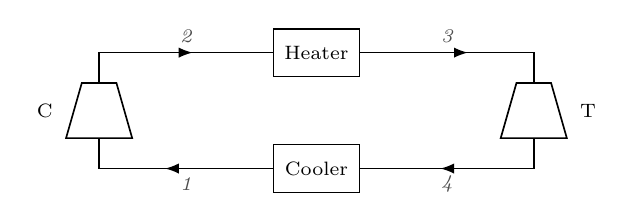
\begin{tikzpicture}[scale=0.92]
\def\yt{1.6}
\draw[fl] (0,0.8)--(0,\yt)--(3,\yt); \draw[fl] (3,\yt)--(6,\yt)--(6,0.8);
\draw[fl] (6,0.8)--(6,0)--(3,0); \draw[fl] (3,0)--(0,0)--(0,0.8);
\pic[rotate=90] at (0,0.8) {comp}; \node[nm] at (-0.75,0.8) {C};
\pic[rotate=-90] at (6,0.8) {turb}; \node[nm] at (6.75,0.8) {T};
\node[box] at (3,\yt) {Heater}; \node[box] at (3,0) {Cooler};
\node[st] at (1.2,\yt+0.22) {2}; \node[st] at (4.8,\yt+0.22) {3};
\node[st] at (4.8,-0.22) {4}; \node[st] at (1.2,-0.22) {1};
\end{tikzpicture}
\caption{Layout 1, simple cycle.}
\end{figure}

Compress, heat, expand, reject. No heat is recovered. The turbine exhaust is still hot, and all of that heat goes to the cooler. \emph{Expected:} the lowest efficiency and the largest cooler duty, but the least hardware. It is the reference that shows what recuperation is worth.

\code{\path{brayton_cycle/simple.py}}

%---------------------------------------------------------------
\subsection{Layout 2: recuperated cycle (the baseline)}
\begin{figure}[h]\centering
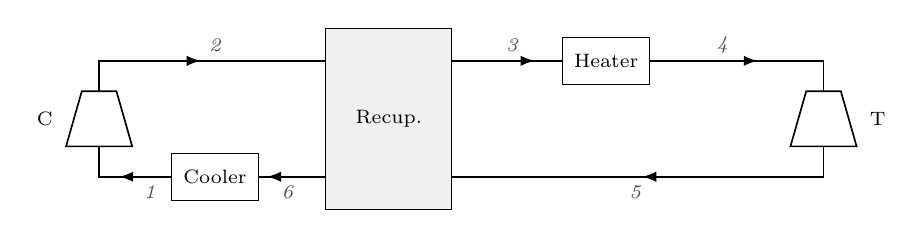
\begin{tikzpicture}[scale=0.92]
\def\yt{1.6}
\draw[fl] (0,0.8)--(0,\yt)--(3.2,\yt); \draw[fl] (4.8,\yt)--(7,\yt); \draw[fl] (7,\yt)--(10,\yt)--(10,0.8);
\draw[fl] (10,0.8)--(10,0)--(4.8,0); \draw[fl] (3.2,0)--(1.6,0); \draw[fl] (1.6,0)--(0,0)--(0,0.8);
\node[hx,minimum width=1.6cm,minimum height=2.3cm] at (4,0.8) {Recup.};
\pic[rotate=90] at (0,0.8) {comp}; \node[nm] at (-0.75,0.8) {C};
\pic[rotate=-90] at (10,0.8) {turb}; \node[nm] at (10.75,0.8) {T};
\node[box] at (7,\yt) {Heater}; \node[box] at (1.6,0) {Cooler};
\node[st] at (1.6,\yt+0.22) {2}; \node[st] at (5.7,\yt+0.22) {3}; \node[st] at (8.6,\yt+0.22) {4};
\node[st] at (7.4,-0.22) {5}; \node[st] at (2.6,-0.22) {6}; \node[st] at (0.7,-0.22) {1};
\end{tikzpicture}
\caption{Layout 2, recuperated cycle.}
\end{figure}

A recuperator uses the turbine exhaust to preheat the compressed stream, so the reactor supplies less heat for the same work. \emph{Expected:} a large gain over layout~1, limited by the heat-capacity mismatch of Section~2: the cold stream needs more heat per kelvin than the hot stream gives up, so the hot stream leaves the recuperator well above the cold inlet temperature and that heat is rejected.

\code{\path{brayton_cycle/recuperated.py}}

%---------------------------------------------------------------
\subsection{Layout 3: recompression cycle}
\begin{figure}[h]\centering
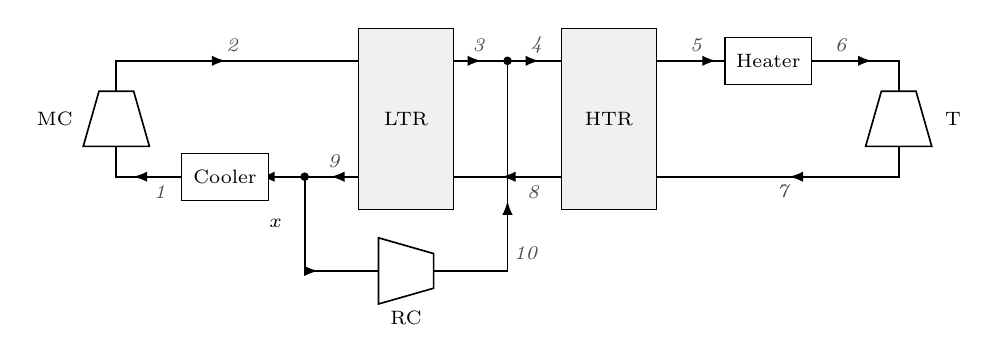
\begin{tikzpicture}[scale=0.92]
\def\yt{1.6}
\draw[fl] (0,0.8)--(0,\yt)--(3.4,\yt); \draw[fl] (4.6,\yt)--(5.4,\yt); \draw[fl] (5.4,\yt)--(6.2,\yt);
\draw[fl] (7.4,\yt)--(9,\yt); \draw[fl] (9,\yt)--(10.8,\yt)--(10.8,0.8);
\draw[fl] (10.8,0.8)--(10.8,0)--(7.4,0); \draw[fl] (6.2,0)--(4.6,0); \draw[fl] (3.4,0)--(2.6,0);
\draw[fl] (2.6,0)--(1.5,0); \draw[fl] (1.5,0)--(0,0)--(0,0.8);
\draw[fl] (2.6,0)--(2.6,-1.3)--(4,-1.3); \draw[fl] (4,-1.3)--(5.4,-1.3)--(5.4,\yt);
\node[hx,minimum width=1.2cm,minimum height=2.3cm] at (4,0.8) {LTR};
\node[hx,minimum width=1.2cm,minimum height=2.3cm] at (6.8,0.8) {HTR};
\pic[rotate=90] at (0,0.8) {comp}; \node[nm] at (-0.85,0.8) {MC};
\pic at (4,-1.3) {comp}; \node[nm] at (4,-1.95) {RC};
\pic[rotate=-90] at (10.8,0.8) {turb}; \node[nm] at (11.55,0.8) {T};
\node[box] at (9,\yt) {Heater}; \node[box] at (1.5,0) {Cooler};
\node[dot] at (2.6,0) {}; \node[dot] at (5.4,\yt) {};
\node[st] at (1.6,\yt+0.22) {2}; \node[st] at (5.0,\yt+0.22) {3}; \node[st] at (5.8,\yt+0.22) {4};
\node[st] at (8.0,\yt+0.22) {5}; \node[st] at (10.0,\yt+0.22) {6};
\node[st] at (9.2,-0.22) {7}; \node[st] at (5.75,-0.22) {8}; \node[st] at (3.0,0.22) {9};
\node[st] at (0.6,-0.22) {1}; \node[st] at (5.65,-1.05) {10};
\node[nm,anchor=north] at (2.2,-0.45) {$x$};
\end{tikzpicture}
\caption{Layout 3, recompression. A fraction $x$ of the flow bypasses the cooler and the main compressor (MC) and is compressed by the recompressor (RC).}\label{fig:l3}
\end{figure}

The recuperator is divided into a low-temperature part (LTR) and a high-temperature part (HTR). After the LTR, a fraction $x$ of the low-pressure flow is sent to a recompressor without being cooled, and rejoins the main flow between the two recuperators. The cold side of the LTR then carries only $(1-x)$ of the flow, which brings its capacity rate down towards that of the hot side. \emph{Expected:} higher efficiency than layout~2, because more heat is recovered and less is rejected. The cost is one more compressor, a second recuperator, and a recompressor that works on warm, less dense fluid. Those two effects pull in opposite directions, so an optimum split fraction should exist.

\code{\path{brayton_cycle/recompression.py}}

%---------------------------------------------------------------
\subsection{Layout 4: recuperated cycle with intercooling}
\begin{figure}[h]\centering
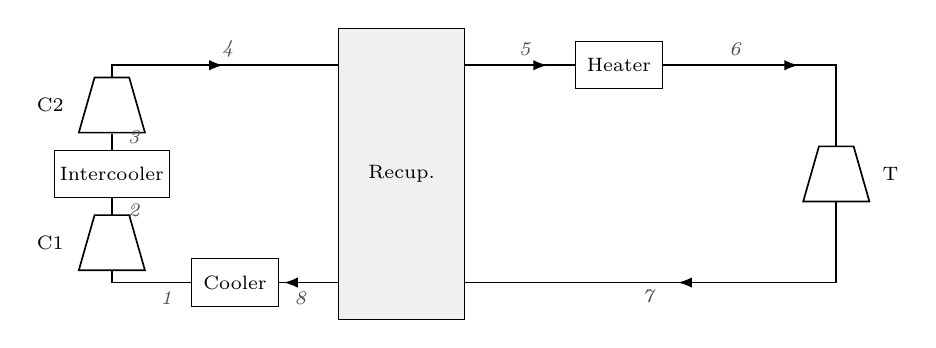
\begin{tikzpicture}[scale=0.92]
\def\yt{3.0}
\draw[fl] (0,0)--(0,1.05); \draw[fl] (0,0.9)--(0,2.05);
\draw[fl] (0,2.5)--(0,\yt)--(3.2,\yt); \draw[fl] (4.8,\yt)--(7,\yt); \draw[fl] (7,\yt)--(10,\yt)--(10,1.5);
\draw[fl] (10,1.5)--(10,0)--(4.8,0); \draw[fl] (3.2,0)--(1.7,0); \draw[ln] (1.7,0)--(0,0);
\node[hx,minimum width=1.6cm,minimum height=3.7cm] at (4,1.5) {Recup.};
\pic[rotate=90] at (0,0.55) {comp}; \node[nm] at (-0.85,0.55) {C1};
\node[box] at (0,1.5) {Intercooler};
\pic[rotate=90] at (0,2.45) {comp}; \node[nm] at (-0.85,2.45) {C2};
\pic[rotate=-90] at (10,1.5) {turb}; \node[nm] at (10.75,1.5) {T};
\node[box] at (7,\yt) {Heater}; \node[box] at (1.7,0) {Cooler};
\node[st] at (1.6,\yt+0.22) {4}; \node[st] at (5.7,\yt+0.22) {5}; \node[st] at (8.6,\yt+0.22) {6};
\node[st] at (7.4,-0.22) {7}; \node[st] at (2.6,-0.22) {8}; \node[st] at (0.75,-0.22) {1};
\node[st] at (0.3,1.0) {2}; \node[st] at (0.3,2.0) {3};
\end{tikzpicture}
\caption{Layout 4, recuperated cycle with two compression stages and an intercooler at $\Pm$.}
\end{figure}

Compression is done in two stages with cooling between them, so the second stage compresses denser fluid and takes less work. \emph{Expected:} lower compressor work than layout~2, but a smaller benefit than in an ideal-gas cycle, because \scotwo{} compression work is already small. Intercooling also lowers the temperature at which the cold stream enters the recuperator. Whether the net effect is a gain is something to compute. The cost is one more compressor and one more cooler.

\code{\path{brayton_cycle/intercooled.py}}

%---------------------------------------------------------------
\subsection{Layout 5: recompression cycle with intercooling}
This is the recompression cycle (layout~3) with the main compression split into two intercooled stages. The recompressor is unchanged.
\begin{figure}[h]\centering
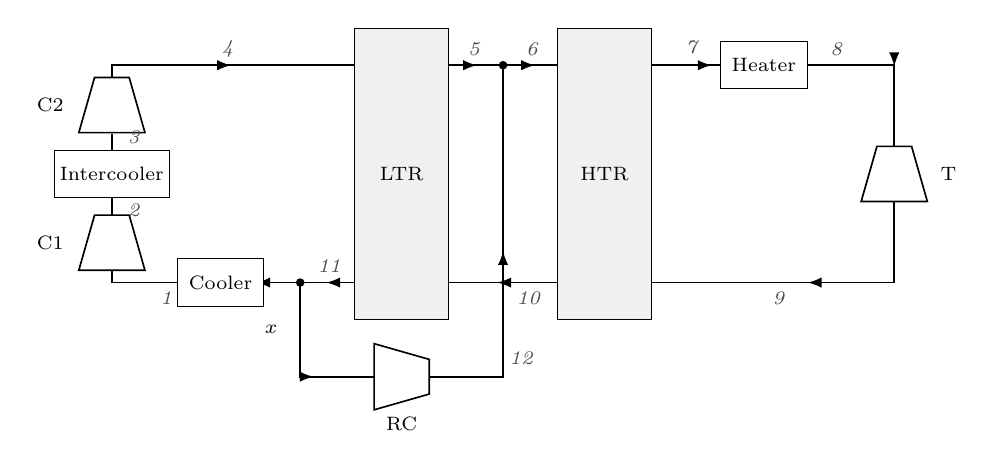
\begin{tikzpicture}[scale=0.92]
\def\yt{3.0}
\draw[fl] (0,0)--(0,1.05); \draw[fl] (0,0.9)--(0,2.05);
\draw[fl] (0,2.5)--(0,\yt)--(3.4,\yt); \draw[fl] (4.6,\yt)--(5.4,\yt); \draw[fl] (5.4,\yt)--(6.2,\yt);
\draw[fl] (7.4,\yt)--(9,\yt); \draw[fl] (9,\yt)--(10.8,\yt)--(10.8,1.5);
\draw[fl] (10.8,1.5)--(10.8,0)--(7.4,0); \draw[fl] (6.2,0)--(4.6,0); \draw[fl] (3.4,0)--(2.6,0);
\draw[fl] (2.6,0)--(1.5,0); \draw[ln] (1.5,0)--(0,0);
\draw[fl] (2.6,0)--(2.6,-1.3)--(4,-1.3); \draw[fl] (4,-1.3)--(5.4,-1.3)--(5.4,\yt);
\node[hx,minimum width=1.2cm,minimum height=3.7cm] at (4,1.5) {LTR};
\node[hx,minimum width=1.2cm,minimum height=3.7cm] at (6.8,1.5) {HTR};
\pic[rotate=90] at (0,0.55) {comp}; \node[nm] at (-0.85,0.55) {C1};
\node[box] at (0,1.5) {Intercooler};
\pic[rotate=90] at (0,2.45) {comp}; \node[nm] at (-0.85,2.45) {C2};
\pic at (4,-1.3) {comp}; \node[nm] at (4,-1.95) {RC};
\pic[rotate=-90] at (10.8,1.5) {turb}; \node[nm] at (11.55,1.5) {T};
\node[box] at (9,\yt) {Heater}; \node[box] at (1.5,0) {Cooler};
\node[dot] at (2.6,0) {}; \node[dot] at (5.4,\yt) {};
\node[st] at (1.6,\yt+0.22) {4}; \node[st] at (5.0,\yt+0.22) {5}; \node[st] at (5.8,\yt+0.22) {6};
\node[st] at (8.0,\yt+0.22) {7}; \node[st] at (10.0,\yt+0.22) {8};
\node[st] at (9.2,-0.22) {9}; \node[st] at (5.75,-0.22) {10}; \node[st] at (3.0,0.22) {11};
\node[st] at (0.75,-0.22) {1}; \node[st] at (0.3,1.0) {2}; \node[st] at (0.3,2.0) {3}; \node[st] at (5.65,-1.05) {12};
\node[nm,anchor=north] at (2.2,-0.45) {$x$};
\end{tikzpicture}
\caption{Layout 5, recompression with an intercooled main compressor.}
\end{figure}

This combines layouts~3 and~4. \emph{Expected:} the efficiency of recompression with slightly lower main-compressor work. It carries the most turbomachinery of the two-pressure layouts (three compressors) and two coolers, so it tests whether the last increment of efficiency pays for its hardware.

\code{\path{brayton_cycle/recomp_intercooled.py}}

%---------------------------------------------------------------
\subsection{Layout 6: partial cooling cycle (Angelino)}
\begin{figure}[h]\centering
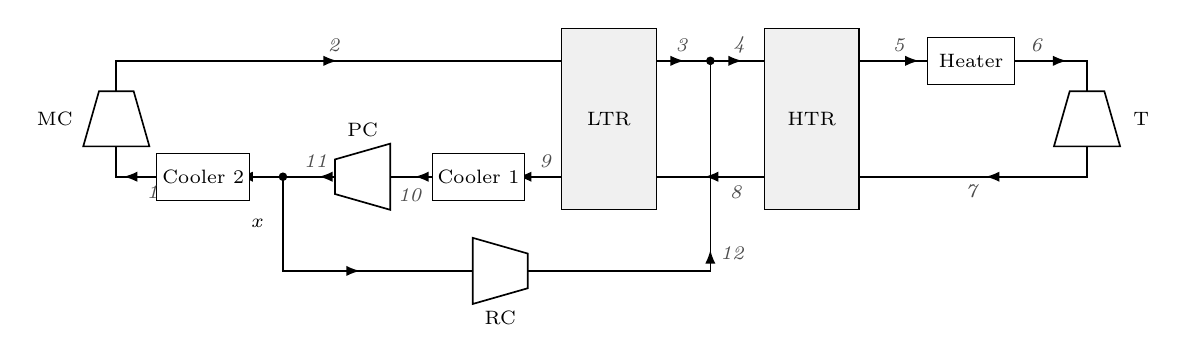
\begin{tikzpicture}[scale=0.92]
\def\yt{1.6}
\draw[fl] (0,0.8)--(0,\yt)--(6.2,\yt); \draw[fl] (7.4,\yt)--(8.2,\yt); \draw[fl] (8.2,\yt)--(9.0,\yt);
\draw[fl] (10.2,\yt)--(11.8,\yt); \draw[fl] (11.8,\yt)--(13.4,\yt)--(13.4,0.8);
\draw[fl] (13.4,0.8)--(13.4,0)--(10.2,0); \draw[fl] (9.0,0)--(7.4,0); \draw[fl] (6.2,0)--(5.0,0);
\draw[fl] (5.0,0)--(3.4,0); \draw[fl] (3.4,0)--(2.3,0); \draw[fl] (2.3,0)--(1.2,0); \draw[fl] (1.2,0)--(0,0)--(0,0.8);
\draw[fl] (2.3,0)--(2.3,-1.3)--(5.3,-1.3); \draw[fl] (5.3,-1.3)--(8.2,-1.3)--(8.2,\yt);
\node[hx,minimum width=1.2cm,minimum height=2.3cm] at (6.8,0.8) {LTR};
\node[hx,minimum width=1.2cm,minimum height=2.3cm] at (9.6,0.8) {HTR};
\pic[rotate=90] at (0,0.8) {comp}; \node[nm] at (-0.85,0.8) {MC};
\pic[rotate=180] at (3.4,0) {comp}; \node[nm] at (3.4,0.65) {PC};
\pic at (5.3,-1.3) {comp}; \node[nm] at (5.3,-1.95) {RC};
\pic[rotate=-90] at (13.4,0.8) {turb}; \node[nm] at (14.15,0.8) {T};
\node[box] at (11.8,\yt) {Heater};
\node[box,minimum width=9mm] at (5.0,0) {Cooler 1}; \node[box,minimum width=9mm] at (1.2,0) {Cooler 2};
\node[dot] at (2.3,0) {}; \node[dot] at (8.2,\yt) {};
\node[st] at (3.0,\yt+0.22) {2}; \node[st] at (7.8,\yt+0.22) {3}; \node[st] at (8.6,\yt+0.22) {4};
\node[st] at (10.8,\yt+0.22) {5}; \node[st] at (12.7,\yt+0.22) {6};
\node[st] at (11.8,-0.22) {7}; \node[st] at (8.55,-0.22) {8}; \node[st] at (5.92,0.22) {9};
\node[st] at (4.05,-0.25) {10}; \node[st] at (2.75,0.22) {11}; \node[st] at (0.5,-0.22) {1}; \node[st] at (8.5,-1.05) {12};
\node[nm,anchor=north] at (1.95,-0.45) {$x$};
\end{tikzpicture}
\caption{Layout 6, partial cooling. The turbine exhausts to $\Pe$, below the main-compressor inlet pressure $\Pm$. A pre-compressor (PC) raises the full flow from $\Pe$ to $\Pm$ before the split.}
\end{figure}

This layout, due to Angelino~\cite{angelino} and analysed for nuclear use by Dostal~\cite{dostal}, has three pressure levels. The turbine expands to a pressure $\Pe$ below the main-compressor inlet. The full flow is cooled, raised to $\Pm$ by a pre-compressor, and then split as in recompression: one part is cooled again and goes to the main compressor, the other goes to the recompressor. \emph{Expected:} more turbine work per kilogram, because of the larger expansion ratio, with the mismatch in the LTR reduced as in layout~3. The cost is three compressors and two coolers.

\code{\path{brayton_cycle/partial_cooling.py}}

%---------------------------------------------------------------
\subsection{Summary of hardware and free variables}

\begin{table}[h]\centering\small\setlength{\tabcolsep}{3.5pt}
\begin{tabular}{clcccl}
\toprule
\# & Layout & Compressors & Recuperators & Coolers & Swept variables\\
\midrule
1 & Simple & 1 & 0 & 1 & $\Ph,\ \Pl,\ \Tin,\ \Tt$\\
2 & Recuperated & 1 & 1 & 1 & $\Ph,\ \Pl,\ \Tin,\ \Tt$\\
3 & Recompression & 2 & 2 & 1 & $\Ph,\ \Pl,\ \Tin,\ \Tt,\ x$\\
4 & Recuperated + intercooling & 2 & 1 & 2 & $\Ph,\ \Pl,\ \Tin,\ \Tt,\ \Pm$\\
5 & Recompression + intercooling & 3 & 2 & 2 & $\Ph,\ \Pl,\ \Tin,\ \Tt,\ \Pm,\ x$\\
6 & Partial cooling & 3 & 2 & 2 & $\Ph,\ \Pm,\ \Pe,\ \Tin,\ \Tt,\ x$\\
\bottomrule
\end{tabular}
\caption{Hardware count and operating variables of each layout. $\Ph$ is the compressor outlet pressure, $\Pl$ the main-compressor inlet pressure, $\Tin$ the compressor inlet temperature, $\Tt$ the turbine inlet temperature and $x$ the split fraction.}\label{tab:layouts}
\end{table}

Pressure ratios are not set directly. Each compressor's ratio follows from the pressure levels on either side of it.

\code{\path{helpers/builders.py} (numbers for each layout), \path{grids.py} (swept variables)}

\section{Thermodynamic model}\label{sec:model}

Each layout is a set of components connected by streams. A stream is described by its pressure and specific enthalpy. All other properties come from CoolProp. This section gives the model of each component. Appendix~\ref{app:numerics} gives the numerical details and Appendix~\ref{app:validation} the validation.

\subsection{Compressor and turbine}
The isentropic outlet enthalpy $h_s$ is the enthalpy at the outlet pressure and the inlet entropy. The actual outlet follows from the isentropic efficiency:
\begin{align}
\text{compressor:}\quad h_\mathrm{out} &= h_\mathrm{in} + \frac{h_s - h_\mathrm{in}}{\eta_c}, &
\text{turbine:}\quad h_\mathrm{out} &= h_\mathrm{in} - \eta_t\,(h_\mathrm{in} - h_s).
\end{align}

\code{\path{cycles/blocks/compressor.py}, \path{cycles/blocks/turbine.py}, \path{cycles/physics/isentropic.py}}

\subsection{Heater and mass flow}
The heater raises the stream to the turbine inlet temperature $\Tt$ at constant pressure. The reactor power is fixed, so the mass flow follows from the heater's enthalpy rise:
\begin{equation}
\dot m = \frac{\dot Q_\mathrm{th}}{h_\mathrm{heater,out} - h_\mathrm{heater,in}}, \qquad \dot Q_\mathrm{th} = \SI{100}{MW}.
\end{equation}

\code{\path{cycles/blocks/heater.py}, \path{cycles/solve.py}}

\subsection{Recuperator}\label{sec:recup}
\paragraph{Effectiveness.} With a varying $c_p$, the maximum heat transfer has to be written in enthalpy. Two limits apply: the hot stream cannot leave colder than the cold stream enters, and the cold stream cannot leave hotter than the hot stream enters.
\begin{equation}
\dot Q_\mathrm{max} = \min\Big[\ \dot m_h\big(h_{h,\mathrm{in}} - h(P_h,\,T_{c,\mathrm{in}})\big),\ \ \dot m_c\big(h(P_c,\,T_{h,\mathrm{in}}) - h_{c,\mathrm{in}}\big)\Big]
\end{equation}
The effectiveness is $\varepsilon = \dot Q/\dot Q_\mathrm{max}$, and it is fixed at the given baseline value, $\varepsilon = 0.90$. The duty $\dot Q = \varepsilon\,\dot Q_\mathrm{max}$ then gives both outlet enthalpies by energy balance.

\paragraph{Pinch.} The minimum temperature difference can occur inside the exchanger, not only at an end, because $c_p$ varies. The exchanger is divided into $N = 100$ slices of equal heat duty. At each of the $N+1$ boundaries the enthalpy of both streams is known from the energy balance, and the temperatures follow from $T(P,h)$. The pinch is the smallest temperature difference found:
\begin{equation}
\Delta T_\mathrm{pinch} = \min_{j}\,\big(T_{h,j} - T_{c,j}\big).
\end{equation}
A design with $\Delta T_\mathrm{pinch} < \SI{5}{K}$ in any recuperator is rejected as infeasible.

\paragraph{Conductance.} A single log-mean temperature difference is valid only when $c_p$ is constant. Here each slice is short enough to treat that way, and the slice conductances are added:
\begin{equation}
UA = \sum_{j=1}^{N} \frac{\Delta \dot Q}{\Delta T_{\mathrm{lm},j}}, \qquad
\Delta T_{\mathrm{lm},j} = \frac{\Delta T_j - \Delta T_{j-1}}{\ln\left(\Delta T_j/\Delta T_{j-1}\right)}, \qquad \Delta\dot Q = \frac{\dot Q}{N}.
\end{equation}
$UA$ is the measure of exchanger size used for mass.

\code{\path{cycles/blocks/heat_exchanger.py}, \path{cycles/physics/hx_limits.py}, \path{cycles/physics/hx_profile.py}, \path{cycles/physics/hx_sizing.py}}

\subsection{Coolers}\label{sec:cooler}
Each cooler brings the \cotwo{} to the compressor inlet temperature $\Tin$, so its duty is fixed by the cycle. The cooling-water supply temperature is given (\SI{25}{\celsius}) but not the water flow, and the size of the cooler depends on that flow. More water keeps the water colder, which widens the temperature difference and shrinks the exchanger.

The water flow is set by a design rule: \emph{the minimum temperature difference between \cotwo{} and water is \SI{5}{K}}. For a trial water flow $\dot m_w$, the water outlet enthalpy follows from the energy balance, and the temperature profile is built in the same $N$ equal-duty slices as the recuperator. The water flow is adjusted by bisection until the smallest temperature difference equals \SI{5}{K}. The cooler's $UA$ is then computed from that profile with the same summation as above.

The order of calculation is: duty (from the cycle) $\rightarrow$ water flow (from the pinch rule) $\rightarrow$ temperature profile $\rightarrow$ $UA$. No value has to be guessed.

\code{\path{cycles/blocks/cooler.py}, \path{cycles/physics/coolant.py}}

\subsection{Pressures}
Pressure drops are not modelled (Section~\ref{sec:limits}). The heater, both sides of each recuperator and the coolers are at constant pressure, and only the compressors and the turbine change it. The compressor outlet, heater and turbine inlet are therefore all at $\Ph$, and the limit of \SI{20}{MPa} applies to $\Ph$.

\code{\path{cycles/passes/pressure.py}}

\subsection{Flow splitting and mixing}
\paragraph{Splitter.} A splitter divides one stream into two at the same state. Nothing thermodynamic happens in it: both outlets keep the inlet pressure and enthalpy, and only the mass flow is divided. With $\dot m$ the inlet flow and $x$ the split fraction sent to the recompressor,
\begin{equation}
\dot m_\mathrm{main} = (1 - x)\,\dot m, \qquad \dot m_\mathrm{RC} = x\,\dot m, \qquad h_\mathrm{main} = h_\mathrm{RC} = h_\mathrm{in}.
\end{equation}

\paragraph{Mixer.} A mixer joins two streams at the same pressure. It is adiabatic and does no work, so the energy balance gives the outlet enthalpy as the flow-weighted mean of the inlets:
\begin{equation}
\dot m_\mathrm{out} = \dot m_1 + \dot m_2, \qquad h_\mathrm{out} = \frac{\dot m_1 h_1 + \dot m_2 h_2}{\dot m_1 + \dot m_2}.
\end{equation}
In the recompression cycle the mixer joins the main flow leaving the low-temperature recuperator with the recompressor outlet. The two are generally at different temperatures, and the outlet temperature is found from $(P, h_\mathrm{out})$ through the property routines. The solver checks that the inlet pressures agree, since a mismatch would mean the layout is wired wrongly.

\paragraph{Why the flow-splitting layouts are iterative.} In the simple and recuperated layouts every component can be evaluated in one pass, each after the components that feed it. In layouts~3, 5 and~6 this is not possible, because the two recuperators and the mixer form a loop. In the recompression cycle (Figure~\ref{fig:l3}):
\begin{itemize}
  \item the low-temperature recuperator needs its hot inlet, which is the hot outlet of the high-temperature recuperator;
  \item the high-temperature recuperator needs its cold inlet, which is the mixer outlet;
  \item the mixer needs the cold outlet of the low-temperature recuperator and the recompressor outlet, and the recompressor takes its inlet from the hot outlet of the low-temperature recuperator.
\end{itemize}
Each of the three needs the result of another before it can be evaluated. The turbine is outside the loop: its inlet is fixed by $\Ph$ and $\Tt$, so its outlet, which is the hot inlet of the high-temperature recuperator, is known from the start.

\paragraph{How the loop is solved.} The loop is broken by guessing one stream, the hot inlet of the low-temperature recuperator, and solved by successive substitution:
\begin{enumerate}
  \item Guess the enthalpy of that stream. The first guess is taken at a temperature a quarter of the way from the compressor inlet temperature to the turbine inlet temperature, which places it in the right region of the property surface.
  \item Evaluate every component in order around the cycle with this guess: low-temperature recuperator, splitter, cooler and recompressor, mixer, high-temperature recuperator.
  \item The high-temperature recuperator returns a new value of the guessed enthalpy. Compare it with the guess.
  \item If the relative change is below $10^{-8}$, stop. Otherwise replace the guess with the new value and repeat from step~2.
\end{enumerate}
The iteration converges because the loop corrects itself: a guess that is too high returns a lower value, and a guess that is too low returns a higher one. It typically settles in about thirty passes. A design that does not converge within 200 passes is flagged and recorded as not solved, rather than stopping the sweep. Layouts~5 and~6 contain the same recuperator--mixer loop and are solved the same way.

\code{\path{cycles/blocks/splitter.py}, \path{cycles/blocks/mixer.py}, \path{cycles/physics/mixing.py}, \path{cycles/passes/flow.py}, \path{cycles/passes/ordering.py}, \path{cycles/passes/tear.py}}

\subsection{Cycle performance}
\begin{align}
\eta &= \frac{\dot W_\mathrm{turb} - \sum \dot W_\mathrm{comp}}{\dot Q_\mathrm{th}}, &
\eta_\mathrm{Carnot} &= 1 - \frac{\Tin}{\Tt}\ \ \text{(in kelvin)}, &
\eta_\mathrm{II} &= \frac{\eta}{\eta_\mathrm{Carnot}}.
\end{align}
The Carnot efficiency is evaluated for each design from its own turbine inlet and compressor inlet temperatures. The second-law efficiency $\eta_\mathrm{II}$ is reported and not optimised.

\code{\path{cycles/result.py}, \path{helpers/checks.py}}

\section{Objective and method}\label{sec:objective}

\subsection{What is computed}
The cycle model gives two engineering quantities for each design: the \textbf{thermal efficiency} $\eta$ and the \textbf{conductance} $UA$ of every heat exchanger. Efficiency sets the electricity produced. Conductance sets the size of the exchangers, and from it the mass and cost of the hardware.

\code{\path{core/solve_points.py}, \path{core/economics.py}}

\subsection{Constraints}
A design is feasible only if it meets all the given limits (Table~\ref{tab:constraints}).

\begin{table}[!htbp]\centering\small
\begin{tabular}{ll}
\toprule
Quantity & Limit\\
\midrule
Compressor inlet temperature & $\geq \SI{32}{\celsius}$\\
Compressor inlet pressure & $\geq \SI{7.7}{MPa}$\\
Maximum cycle pressure & $\leq \SI{20}{MPa}$\\
Turbine inlet temperature & $\leq \SI{500}{\celsius}$\\
Recuperator minimum pinch & $\geq \SI{5}{K}$\\
Split fraction & between 0 and 0.5\\
\bottomrule
\end{tabular}
\caption{Given constraints.}\label{tab:constraints}
\end{table}

The compressor inlet limits keep the compressor away from the two-phase region.

In layout~6 the pre-compressor inlet is at $\Pe$, which lies below the main compressor inlet pressure by construction (\SI{4.5}{MPa} to \SI{7.5}{MPa} in the grid). We therefore apply the \SI{7.7}{MPa} limit to the main compressor inlet only, which in layout~6 is at $\Pm$ (\SI{7.7}{MPa} to \SI{8.7}{MPa}) and meets it. Only the pre-compressor, which raises the flow from $\Pe$ to $\Pm$ before the main compressor, operates below the limit. This does not bring the pre-compressor into the two-phase region: two phases coexist only below the critical temperature (\SI{30.98}{\celsius}), and every compressor inlet is at \SI{32}{\celsius} or above, so the inlet is a single-phase gas at every grid point. What is lost is the high density that the limit secures. At \SI{32}{\celsius} the inlet density is \SI{104}{kg/m^3} at \SI{4.5}{MPa} against \SI{602}{kg/m^3} at \SI{7.7}{MPa}, so the pre-compressor needs more work per unit mass. We therefore report the layout~6 results with this exception to the given limits.

\code{\path{config.py} (section B), \path{helpers/checks.py}}

\subsection{Mass}
The given data include one conversion from conductance to mass for a printed-circuit heat exchanger, \SI{2.5}{kg} per \si{kW/K}, an allowance of \SI{1.5}{t} for an added compressor, and a baseline system mass of about \SI{60}{t} for the simple recuperated cycle. The mass of a design is
\begin{equation}
m = k_{UA}\Big(\sum UA_\mathrm{recuperators} + \sum UA_\mathrm{coolers}\Big) + M_0 + m_c\,n_\mathrm{extra},
\end{equation}
with $k_{UA} = \SI{2.5}{kg}$ per \si{kW/K}, $m_c = \SI{1.5}{t}$, and $n_\mathrm{extra}$ the number of compressors beyond the first (Table~\ref{tab:layouts}).

$M_0$ is the fixed mass of the power-conversion system: everything that is not a heat exchanger or an added compressor, namely the turbine, generator, first compressor, piping and structure. The given data do not state this mass directly. They give only a total of about \SI{60}{t} for the baseline recuperated cycle, which includes its recuperator and cooler. We therefore find $M_0$ by calibration, in three steps.
\begin{enumerate}
  \item We sweep the recuperated layout (layout~2) and take its feasible design with the highest efficiency as the reference.
  \item We compute the mass of the reference's two exchangers from their conductance.
  \item We set $M_0$ so that the reference has the given baseline mass:
  \begin{equation}
  M_0 = \SI{60}{t} - k_{UA}\big(UA_\mathrm{recup} + UA_\mathrm{cooler}\big)_\mathrm{reference}.
  \end{equation}
\end{enumerate}
The reference is the layout~2 design at $\Ph = \SI{20}{MPa}$, $\Pl = \SI{7.7}{MPa}$, $\Tin = \SI{34}{\celsius}$ and $\Tt = \SI{500}{\celsius}$. Its efficiency is 33.3\%, and the calibration gives $M_0 = \SI{39.06}{t}$ (Section~\ref{sec:results}). We hold this value fixed for every layout and operating point, so that differences in mass between designs come only from heat-exchanger conductance and added compressors (the limits of this choice are in Section~\ref{sec:limits}). For the same reason, the baseline efficiency we compare against is the computed 33.3\% of the reference, not the placeholder of 30\% in the given worked example.

Volume is taken as mass divided by the baseline density, $\SI{60}{t}/\SI{120}{m^3} = \SI{0.5}{t/m^3}$.

\code{\path{core/calibrate.py}, \path{core/economics.py}}

\subsection{Cost, lifetime payout and incremental payback}
One price is given for installed hardware, \SI{250}{US\$/kg}, and an electricity value of \SI{70}{US\$/MWh} over \SI{7000}{h} per year. Hardware cost is therefore taken as proportional to mass. Two economic measures are used, and neither is a financial result.

\paragraph{Lifetime payout (for ranking).} To put a one-time hardware cost and a yearly income on one scale, every design is given the score
\begin{equation}
\Pi_N = \underbrace{N \,\eta\, \dot Q_\mathrm{th}\, t_\mathrm{op}\, c_e}_{\text{electricity value over } N \text{ years}} \;-\; \underbrace{c_m\, m}_{\text{power-conversion hardware cost}},
\end{equation}
with $t_\mathrm{op} = \SI{7000}{h/yr}$, $c_e = \SI{70}{US\$/MWh}$, $c_m = \SI{250}{US\$/kg}$ and $N = 10$ years. $\Pi_N$ is called the payout in this report, but it is \emph{not} a payout or profit in the financial sense. It leaves out the reactor and heater, fuel, operation and maintenance, financing and construction, and it does not discount future income. Its absolute value therefore means nothing. Only the \emph{difference} in $\Pi_N$ between two designs is used, and that difference is meaningful only to the extent that the omitted costs are the same for both (Section~\ref{sec:limits}). We use $\Pi_N$ because it combines the two quantities the given data do price, efficiency and hardware mass, into one number that rises with efficiency and falls with mass.

\paragraph{Incremental payback (for comparison with the baseline).} The given worked comparison measures a candidate against the baseline: the extra electricity it produces is valued per year, the extra hardware is costed, and the two are compared. The same calculation is used here. For a candidate with efficiency $\eta$ and mass $m$ against the reference with $\eta_\mathrm{ref}$ and $m_\mathrm{ref}$,
\begin{equation}
\Delta \dot V = (\eta - \eta_\mathrm{ref})\,\dot Q_\mathrm{th}\, t_\mathrm{op}\, c_e, \qquad
\Delta C = c_m\,(m - m_\mathrm{ref}), \qquad
t_\mathrm{pb} = \frac{\Delta C}{\Delta \dot V}.
\end{equation}
$t_\mathrm{pb}$ is the time over which the added electricity value equals the added hardware cost. It is a simple, undiscounted comparison of the added hardware with the added output, under the same omissions as $\Pi_N$. It is not the time for the plant to pay for itself, which would need the full plant cost. Whenever this report says that a design ``recovers'' its extra hardware cost in some time, this incremental payback is meant.

\code{\path{core/economics.py}}

\subsection{Selection}
Two objectives are used:
\begin{itemize}
  \item maximise the lifetime payout $\Pi_N$;
  \item minimise the mass $m$, as the measure of compactness.
\end{itemize}

\paragraph{Why two objectives and not one.} Payout already combines efficiency and hardware cost in one number, so efficiency is not a separate objective. Mass is kept as a second objective because a small modular reactor is valued for being compact and transportable, and the price of \SI{250}{US\$/kg} does not capture that. The two conflict whenever extra heat-exchanger area buys extra efficiency: the payout rises and so does the mass. There is then no single best design, only a set of reasonable trade-offs, and the selection has to be made in steps.

\paragraph{Step 1: Pareto front (remove designs that are worse on both).} A design is \emph{dominated} if some other feasible design has a higher payout and a lower mass. Nobody would choose a dominated design, whatever their preference between payout and mass. Removing all dominated designs leaves the Pareto front. Every design on the front is a valid answer to the question ``what is the best payout available at this mass?''. This step uses no weights and no judgement.

\paragraph{Step 2: knee point (the balanced design on the front).} Moving along the front from light to heavy, payout first rises quickly and then flattens. The knee is where the front bends: before it, a little mass buys a lot of payout, and after it, a lot of mass buys little. It is located as follows. Both objectives are scaled to the range 0 to 1 over the front, so that tonnes and dollars can be compared. The ideal corner is the point with the highest payout and the lowest mass on the front, which no real design reaches. The knee is the design on the front with the smallest distance to that corner,
\begin{equation}
d = \sqrt{(1 - \hat\Pi)^2 + \hat m^2},
\end{equation}
where $\hat\Pi$ and $\hat m$ are the scaled payout and mass. The weakness of this rule is that the scaling depends on the two ends of the front. A very light design with a very low payout stretches the scale and moves the knee, even though it is not a serious candidate. We saw this in our first ranking, which included the simple, non-recuperated layout. Its three lightest designs (about \SI{48.6}{t}, payout \$45M to \$60M) formed the light end of the front, and the knee moved to the recuperated reference at \SI{60}{t}. That result reflected the stretched scale rather than any merit of the reference, and it did not help in choosing a design.

\paragraph{Which designs enter the ranking.} For this reason we leave the simple cycle (layout~1) out of the Pareto front, the knee and TOPSIS, while still solving it and reporting its results. It is not a credible candidate in any case: its best efficiency is 15\%, less than half that of the recuperated baseline, and half of its grid could not be solved (Section~\ref{sec:results}). Its role in this study is to show what recuperation is worth, and the comparison of the best design of each layout (Table~\ref{tab:best}) shows that without it.

\paragraph{Step 3: TOPSIS (a ranked list of all designs).} The knee gives one design and says nothing about the next best. TOPSIS ranks every feasible design, on or off the front, and is used as an independent check. Each objective is divided by its root-sum-square over all designs, $r_{ki} = x_{ki}/\sqrt{\sum_k x_{ki}^2}$, and multiplied by a weight, $v_{ki} = w_i r_{ki}$. The ideal design takes the best value of each objective and the worst design the worst value of each. For design $k$, $d_k^{+}$ is its distance to the ideal and $d_k^{-}$ its distance to the worst, and the score is
\begin{equation}
C_k = \frac{d_k^{-}}{d_k^{+} + d_k^{-}}, \qquad 0 \le C_k \le 1 .
\end{equation}
A design scores well if it is close to the ideal and far from the worst. Equal weights, $w = 0.5$ for each objective, are used, because nothing given says that one objective matters more. TOPSIS differs from the knee in two ways: it scales by the whole feasible set and not by the ends of the front, and it rewards distance from the worst design. It is therefore less sensitive to a few extreme designs.

\paragraph{Using the two together.} The knee and TOPSIS are computed independently, so their agreement is a check on the selection. In this study they select the same design (Section~\ref{sec:results}). The selected design is then compared with the best design on each single measure (payout, efficiency and mass) to state what the compromise costs.

The following are also reported for the selected design and for the best design of each layout: specific power (\si{MWe/t} and \si{MWe/m^3}), heat input per \si{MWe}, second-law efficiency, cooling-water flow, and the margin of the compressor inlet above the critical point.

\code{\path{helpers/ranking.py}, \path{core/economics.py}}

\subsection{Fixed parameters}

\begin{table}[!htbp]\centering\small
\begin{tabular}{llr}
\toprule
Group & Parameter & Value\\
\midrule
Given & Reactor thermal power & \SI{100}{MW}\\
 & Compressor isentropic efficiency & 0.89\\
 & Turbine isentropic efficiency & 0.90\\
 & Cooling-water supply temperature & \SI{25}{\celsius}\\
 & Annual operation & \SI{7000}{h}\\
 & Electricity value & \SI{70}{US\$/MWh}\\
 & Installed hardware cost & \SI{250}{US\$/kg}\\
 & Heat-exchanger mass per unit $UA$ & \SI{2.5}{kg} per \si{kW/K}\\
 & Mass of an added compressor & \SI{1.5}{t}\\
 & Baseline system mass and volume & \SI{60}{t}, \SI{120}{m^3}\\
 & Pressure drops & neglected\\
\midrule
Decided & Recuperator effectiveness & 0.90 (held fixed)\\
& Cooler minimum temperature difference & \SI{5}{K}\\
 & Cooler mass per unit $UA$ & same as recuperator\\
 & Cooler outlet temperature & compressor inlet temperature\\
 & Lifetime for payout, $N$ & 10 years\\
 & TOPSIS weights (payout, mass) & 0.5, 0.5\\
\midrule
Calibrated & $M_0$ & \SI{39.06}{t}\\
\bottomrule
\end{tabular}
\caption{Parameters held fixed in every calculation.}\label{tab:config}
\end{table}

\code{\path{config.py}}

\section{Assumptions and limitations}\label{sec:limits}

The given mass and cost figures are illustrative, and several quantities had to be assumed. The study is therefore a first-pass comparison of layouts and not a design calculation. The points below state what we assumed and how it could affect the conclusions.

\paragraph{Cycle model}
\begin{itemize}
  \item \textbf{No pressure drops.} All heat exchangers and pipes are taken as isobaric, so pressure drops are neglected throughout this project. They could be modelled: the solver accepts a pressure drop for each exchanger side (\path{cycles/physics/pressure_drop.py}) and resolves the resulting pressures around the loop, but we set every drop to zero. Real losses of 1--2\% of pressure per exchanger side would lower every efficiency, and would penalise the layouts with more exchangers (layouts 3 to 6) slightly more than the simpler ones.
  \item \textbf{Constant component efficiencies.} The same isentropic efficiencies are used for every compressor and for the turbine, whatever their size, pressure ratio or inlet state.
  \item \textbf{Fixed recuperator effectiveness.} Effectiveness is listed as a design variable. It is held at 0.90 here, and designs whose pinch falls below \SI{5}{K} are rejected.
  \item \textbf{Design point only.} Part-load and off-design operation are not modelled.
\end{itemize}

\paragraph{Coolers}
\begin{itemize}
  \item \textbf{Cooler pinch of \SI{5}{K}.} The water flow is not given. We assume a minimum temperature difference of \SI{5}{K}, which fixes the water flow and the cooler size. A smaller value gives a larger cooler and less water, and a larger value the opposite.
  \item \textbf{No pumping power or pumping hardware.} The water flow that results from the pinch rule is large, and the power to pump it is not subtracted from the net output. The pump and water circuit are not included in the mass. This favours designs that reject more heat.
  \item \textbf{Cooler mass.} The only guidance given is that the precooler scales with heat rejected. The recuperator's figure of \SI{2.5}{kg} per \si{kW/K} is applied to coolers too.
  \item \textbf{Water side.} Cooling water is once-through at \SI{25}{\celsius} and \SI{6}{bar}, with no pressure drop.
\end{itemize}

\paragraph{Mass and cost}
\begin{itemize}
  \item \textbf{Turbomachinery mass does not scale.} $M_0$ is constant across layouts and operating points. In reality the mass of the turbine and compressors depends on mass flow and pressure ratio. With a fixed machine mass, the model has no penalty for a high pressure ratio.
  \item \textbf{One price for all hardware.} Every kilogram costs the same, \SI{250}{US\$/kg}, whether it is a printed-circuit heat exchanger, a cooler, a compressor or the turbine, so hardware cost is proportional to mass. In reality the cost per kilogram differs between component types: turbomachinery, with its bearings, seals and precision parts, costs more per kilogram than a diffusion-bonded heat exchanger. With separate prices, layouts with more compressors (layouts 3, 5 and 6) would be penalised more, and layouts that add exchanger area would be penalised less, than in this study.
  \item \textbf{Heater and reactor excluded.} The reactor thermal power is the same for every design, so we leave the reactor out. The heater duty is also fixed at \SI{100}{MW}, but its inlet temperature differs between designs (it is higher when more heat is recuperated), so its size and cost are not exactly equal. We leave the heater out of mass and cost, which slightly favours designs that recuperate less.
  \item \textbf{Volume carries no independent information.} It is mass divided by a constant density.
  \item \textbf{No operating costs.} The payout counts electricity income and hardware cost only. Maintenance is not included, although it would grow with the number of compressors, seals and exchangers. Fuel and the operation of the reactor and heater are not included either. They are the same for every design only to first order.
  \item \textbf{Fixed prices.} The electricity value of \SI{70}{US\$/MWh}, the \SI{7000}{h} of operation per year and the hardware price are held constant for $N$ years. Any of them may change over a ten-year life. A higher electricity value or a longer life favours the more efficient, heavier designs; a higher hardware price favours the lighter ones.
  \item \textbf{No time value of money.} Income is not discounted and there is no financing, inflation or construction period. A discount rate would weight early years more and act like a shorter $N$.
  \item \textbf{A ranking measure, not a financial one.} For all these reasons the payout and the incremental payback are used only to compare designs with each other and with the baseline. Neither is an estimate of what the plant would earn or when it would pay for itself. The sensitivity of the selection to $N$ is tested in Section~\ref{sec:results}.
  \item \textbf{Complexity is not costed.} More components mean more seals, bearings, controls and failure modes. Only the given \SI{1.5}{t} per added compressor represents this. Where two layouts are close on payout, the simpler one should be preferred.
\end{itemize}

\paragraph{Search}
\begin{itemize}
  \item \textbf{Grid resolution.} The operating variables are swept on a grid, so the optimum is located only to within the grid spacing. The grid is given in Table~\ref{tab:grid}. Around the selected design the split fraction is resolved to 0.01 and the inlet temperature to \SI{1}{K}. Elsewhere the split is resolved to 0.05, the pressures to \SI{0.5}{MPa} to \SI{2}{MPa} and the inlet temperature to \SI{4}{K}.
\end{itemize}

Section~\ref{sec:results} tests the selection against the lifetime $N$ and the grid spacing.

\section{Results}\label{sec:results}

\subsection{Grid and feasible set}
Table~\ref{tab:grid} gives the grid swept for each layout and the number of feasible designs. In total 1053 designs were attempted and 969 were feasible. After the first sweep, we added two refinement grids around the best layout~3 and layout~6 designs. Layout~2 was swept most finely because it sets the calibration. The other layouts were swept at $\Tt = \SI{500}{\celsius}$ only, because the layout~2 sweep showed that efficiency always rises with $\Tt$ (best efficiency 33.3\% at \SI{500}{\celsius}, 32.7\% at \SI{475}{\celsius}, 32.0\% at \SI{451}{\celsius}).

\begin{table}[h]\centering\small
\begin{tabularx}{\textwidth}{@{}c X c c l@{}}
\toprule
Layout & Grid (pressures in MPa, $\Tin$ in \si{\celsius}) & Attempted & Feasible & Rejected\\
\midrule
1 & $\Ph$ 16--20 (step 2); $\Pl$ 7.7, 8.7; $\Tin$ 32, 36, 40 & 18 & 9 & 9 solver error\\
2 & $\Ph$ 14--20 (step 1); $\Pl$ 7.7--9.7 (step 0.5); $\Tin$ 32--40 (step 2); $\Tt$ 500, 475, 451 & 525 & 512 & 13 pinch\\
3 & $\Ph$ 16--20 (step 2); $\Pl$ 7.7, 8.2; $\Tin$ 32, 36, 40; $x$ 0.15--0.40 (step 0.05). Refinement at 20 / 7.7 MPa: $\Tin$ 32, 33, 34; $x$ 0.30--0.40 (step 0.01) & 138 & 136 & 2 pinch\\
4 & as layout 3 without $x$; $\Pm$ 10, 12, 14 & 54 & 53 & 1 cross\\
5 & $\Ph$ 18, 20; $\Pl$ 7.7, 8.2; $\Tin$ 32, 36, 40; $x$ 0.20--0.35; $\Pm$ 10, 12, 14 & 144 & 91 & 44 pinch, 9 cross\\
6 & $\Ph$ 18, 20; $\Pm$ 7.7, 8.2, 8.7; $\Pe$ 5.5, 6.5, 7.5; $\Tin$ 32, 36, 40; $x$ 0.2, 0.3, 0.4. Refinement at 20 / 7.7 MPa: $\Pe$ 4.5, 5.5; $\Tin$ 32, 36; $x$ 0.35, 0.45, 0.50 & 174 & 168 & 6 pinch\\
\bottomrule
\end{tabularx}
\caption{Grid and feasible set per layout. ``Pinch'' means a recuperator temperature difference below \SI{5}{K}. ``Cross'' is a temperature cross, a recuperator pinch below zero.}\label{tab:grid}
\end{table}

\paragraph{Layout 1 limitation.} Nine of the 18 layout~1 designs did not solve. Without a recuperator the cooler receives turbine exhaust at about \SI{400}{\celsius}, and the search for the cooling-water flow reaches the boiling point of water at the solver's coolant pressure of \SI{6}{bar} (\SI{159}{\celsius}). This is a limit of the cooler model, not of the cycle. The nine designs that solved have efficiencies of 10\% to 15\%, far below every other layout, so the missing points cannot change any conclusion.

\code{\path{grids.py}, \path{core/make_inputs.py}, \path{core/solve_points.py}, \path{data/inputs.csv}, \path{data/infeasible.csv}}

\subsection{Calibration}
The most efficient feasible layout~2 design is $\Ph = \SI{20}{MPa}$, $\Pl = \SI{7.7}{MPa}$, $\Tin = \SI{34}{\celsius}$, $\Tt = \SI{500}{\celsius}$, with $\eta = 33.3\%$. Its recuperator has $UA = \SI{1866}{kW/K}$ (\SI{4.66}{t}) and its cooler $UA = \SI{6511}{kW/K}$ (\SI{16.28}{t}), so
\[ M_0 = 60 - 4.66 - 16.28 = \SI{39.06}{t}. \]
The best inlet temperature is \SI{34}{\celsius} and not the \SI{32}{\celsius} limit. At \SI{32}{\celsius} the compressor work is lower, but the recuperator recovers less heat at fixed effectiveness, and the second effect is larger here. This design, called the recuperated reference from here on, is the baseline for every comparison in the rest of the report.

\code{\path{core/calibrate.py}}

\subsection{Efficiency trends}
\begin{figure}[h]\centering
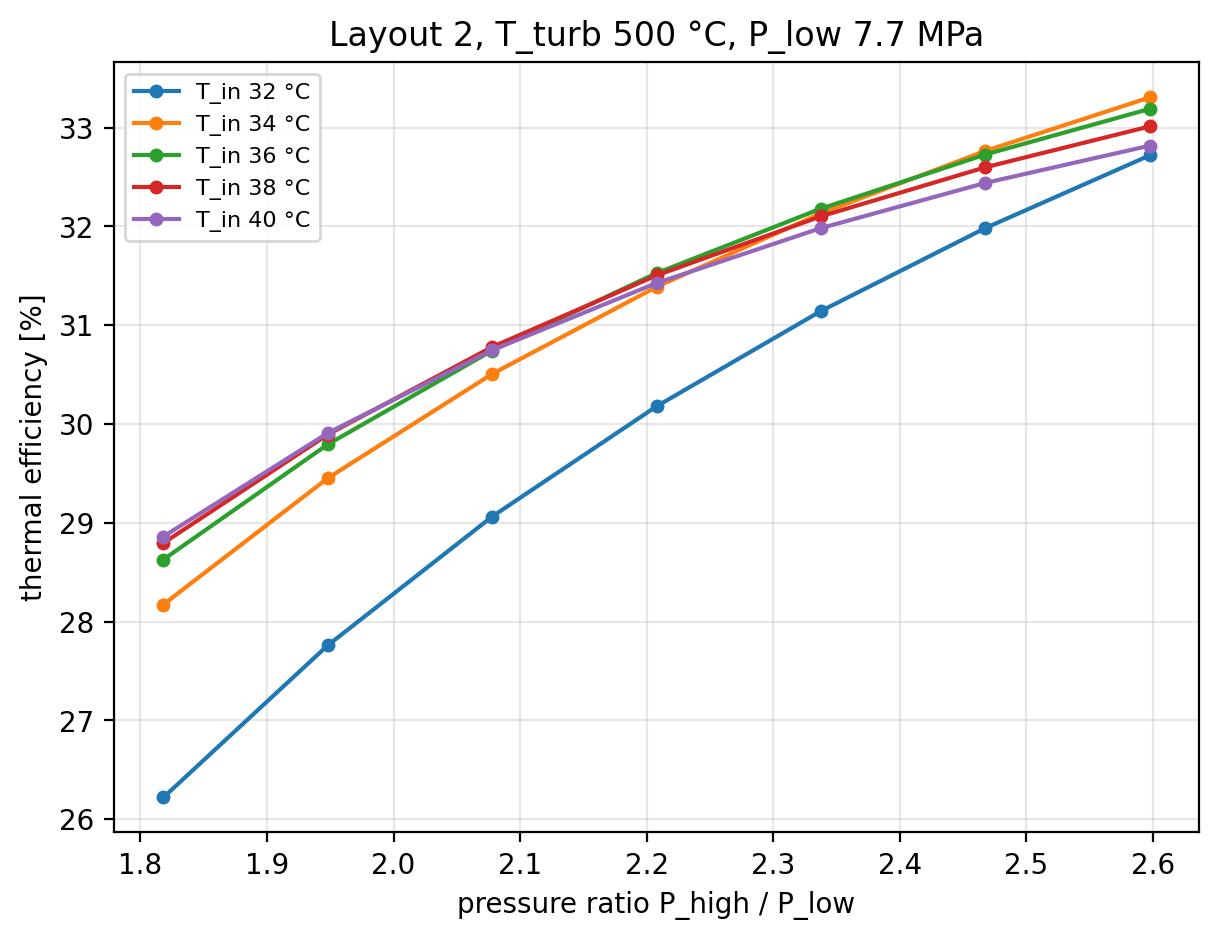
\includegraphics[width=0.49\textwidth]{figs/eta_vs_pressure_ratio.png}\hfill
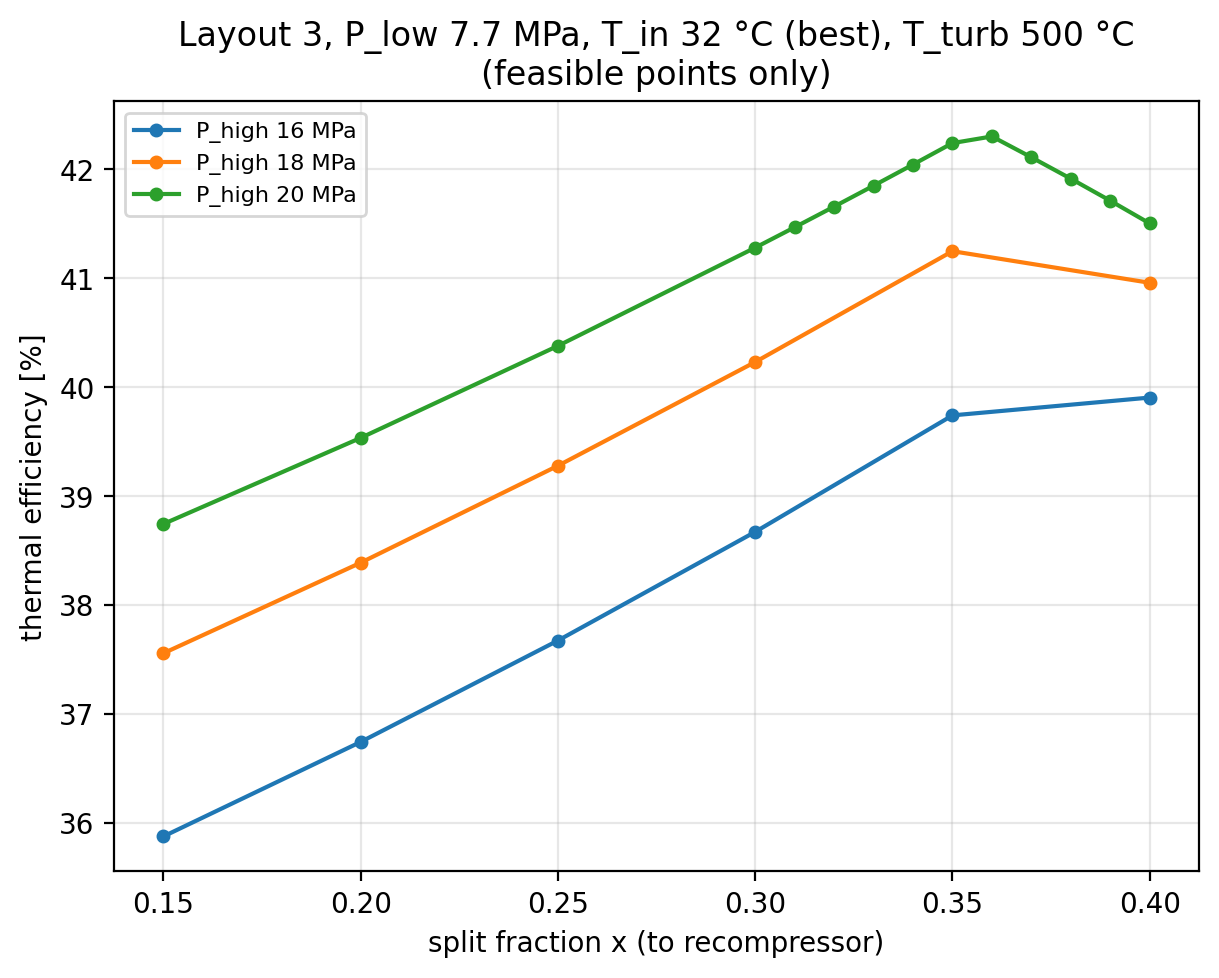
\includegraphics[width=0.49\textwidth]{figs/eta_vs_split.png}
\caption{Efficiency against pressure ratio (left) and against split fraction (right).}\label{fig:trends}
\end{figure}
In every layout the efficiency rises with $\Ph$ up to the \SI{20}{MPa} limit, so the best pressure ratio is the largest one allowed, $20/7.7 = 2.6$. For layout~2 the best efficiency at \SI{500}{\celsius} rises from 28.9\% at \SI{14}{MPa} to 33.3\% at \SI{20}{MPa}. For recompression at \SI{20}{MPa}, \SI{7.7}{MPa} and \SI{32}{\celsius}, efficiency rises with split fraction from 38.7\% at $x = 0.15$ to a maximum of 42.3\% at $x = 0.36$, then falls to 41.5\% at $x = 0.40$. The optimum split for efficiency is 0.36, where the heat capacities of the two streams in the low-temperature recuperator are balanced. Beyond it, the recompressor work grows faster than the heat recovery. The mass also falls beyond 0.36 (from \SI{78.2}{t} to \SI{74.6}{t} at $x = 0.40$), because the temperature difference in the low-temperature recuperator opens from \SI{10}{K} to \SI{18}{K} and it needs less conductance. This is why the rankings that include mass prefer splits above the efficiency optimum.

\code{\path{core/plots.py}, \path{data/results_raw.csv}}

\subsection{Best design of each layout}
\begin{table}[h]\centering\small
\setlength{\tabcolsep}{4pt}\begin{tabular}{@{}clcccccc@{}}
\toprule
Layout & Best design (by payout) & $\eta$ & $\eta_\mathrm{II}$ & $UA$ & Mass & Payout & Sp. power\\
 & & (\%) & (\%) & (kW/K) & (t) & (M\$) & (MWe/t)\\
\midrule
1 & 20 / 7.7 MPa, \SI{32}{\celsius} & 14.8 & 24.5 & 3851 & 48.7 & 60.4 & 0.30\\
2 & 20 / 7.7 MPa, \SI{34}{\celsius} & 33.3 & 55.3 & 8376 & 60.0 & 148.2 & 0.56\\
3 & 20 / 7.7 MPa, \SI{32}{\celsius}, $x = 0.36$ & 42.3 & 69.9 & 15074 & 78.2 & 187.7 & 0.54\\
4 & 20 / 8.2 MPa, \SI{32}{\celsius}, $\Pm = 14$ & 34.1 & 56.3 & 13992 & 75.5 & 148.1 & 0.45\\
5 & 20 / 7.7 MPa, \SI{32}{\celsius}, $\Pm = 10$, $x = 0.35$ & 42.5 & 70.1 & 17763 & 86.5 & 186.4 & 0.49\\
6 & 20 / 7.7 MPa, $\Pe = 5.5$, \SI{32}{\celsius}, $x = 0.45$ & 41.6 & 68.7 & 14110 & 77.3 & 184.5 & 0.54\\
\bottomrule
\end{tabular}
\caption{Best design of each layout by 10-year payout. All at $\Tt = \SI{500}{\celsius}$. Pressures are written as compressor outlet / main compressor inlet ($\Ph$ / $\Pl$). In layout~6 the main compressor inlet is at $\Pm$, and the turbine exhausts to the lower pressure $\Pe$, which is the pre-compressor inlet.}\label{tab:best}
\end{table}

Compared with the expectations of Section~\ref{sec:layouts}:
\begin{itemize}
  \item \textbf{Recuperation is essential.} Layout~1 reaches only 14.8\%. Recuperation more than doubles this for \SI{11}{t} more hardware.
  \item \textbf{Recompression gives the large gain.} Layout~3 adds 9.0 points of efficiency over layout~2. It needs almost twice the conductance, because the two recuperators work at smaller temperature differences.
  \item \textbf{Intercooling does not pay.} Layout~4 gains 0.8 points over layout~2 for \SI{15.5}{t} more mass, and its payout is no better. Layout~5 gains 0.2 points over layout~3 for \SI{8.2}{t} more. \scotwo{} compression near the critical point already takes little work, so there is little left to save.
  \item \textbf{Partial cooling is close to recompression.} Layout~6 reaches 41.6\% at slightly lower mass than the best layout~3 design, but with one more compressor and one more cooler, and its payout is \$3.3M lower. Its pre-compressor inlet is below the \SI{7.7}{MPa} limit in every design (Section~\ref{sec:objective}).
\end{itemize}

\code{\path{core/summary.py}, \path{out/summary.md}}

\subsection{Pareto front, knee and TOPSIS}
\begin{figure}[h]\centering
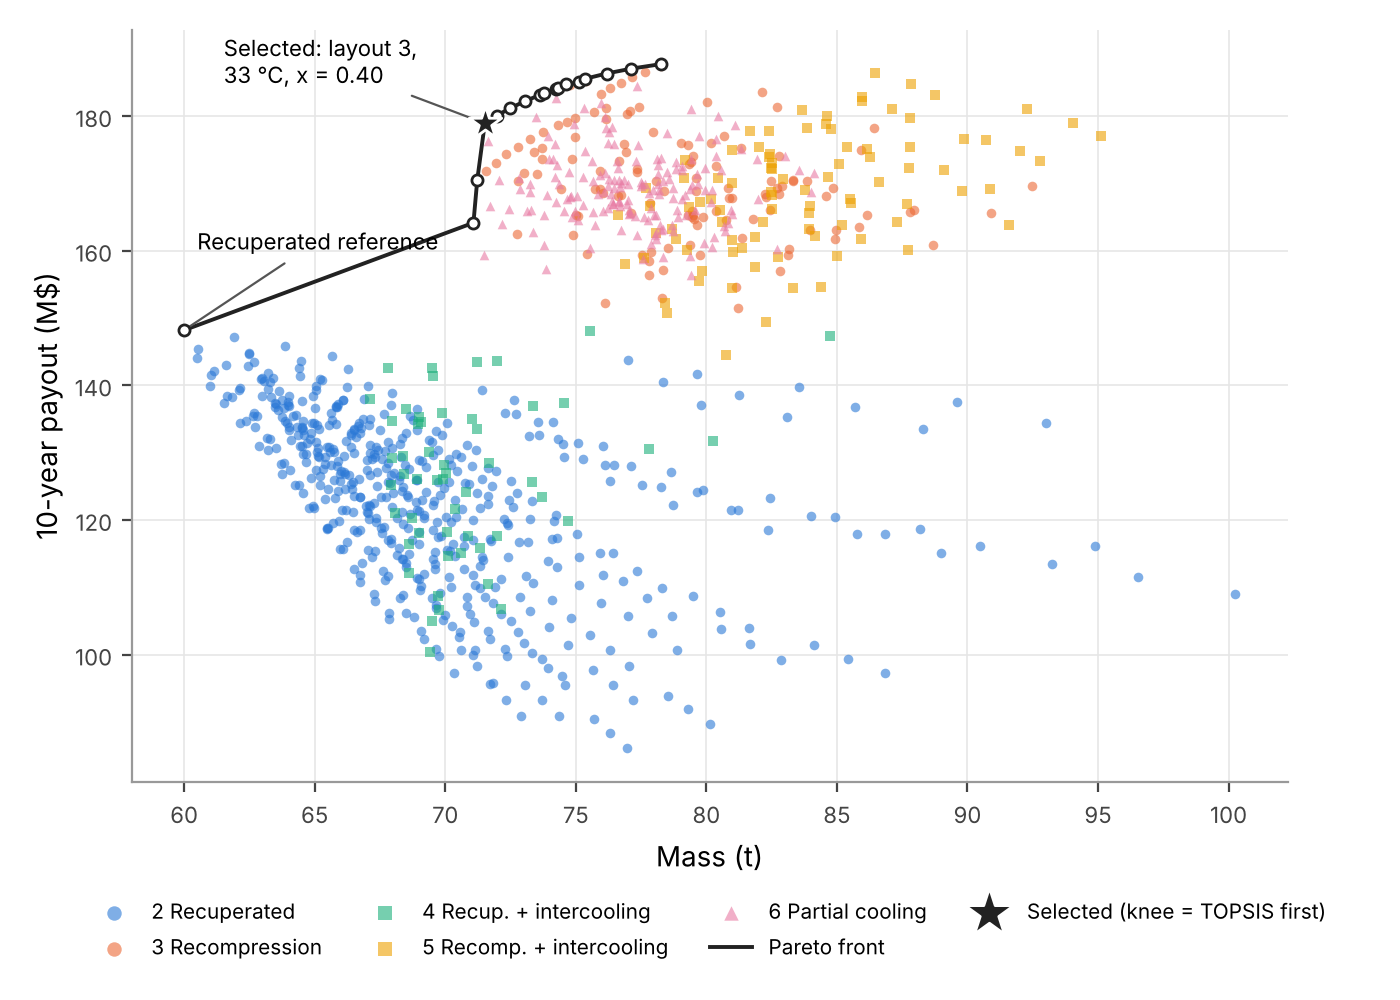
\includegraphics[width=0.82\textwidth]{figs/pareto_noL1.png}
\caption{Ten-year payout against mass for layouts 2 to 6, with the Pareto front and the selected design.}\label{fig:pareto}
\end{figure}
\begin{figure}[h]\centering
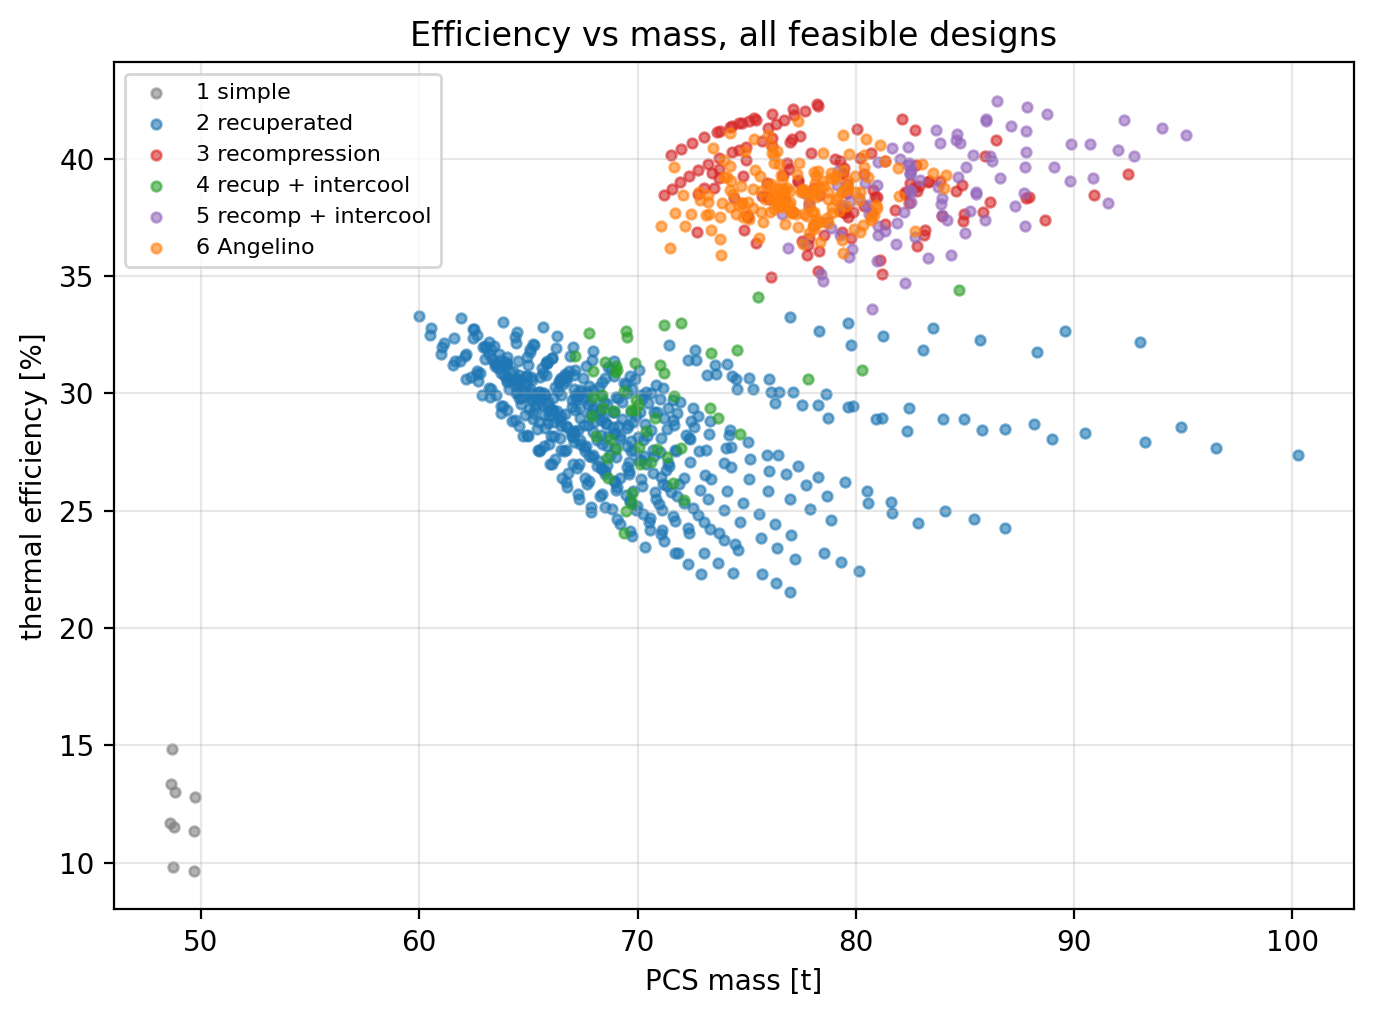
\includegraphics[width=0.6\textwidth]{figs/eta_vs_mass.png}
\caption{Efficiency against mass, all layouts.}\label{fig:etamass}
\end{figure}
With the simple cycle left out (Section~\ref{sec:objective}), 17 designs lie on the Pareto front of payout against mass (Figure~\ref{fig:pareto}). They fall into two groups. The first is the recuperated reference on its own, at \SI{60}{t} and \$148M. The second is sixteen designs between \SI{71}{t} and \SI{78}{t}, with payouts from \$164M to \$188M. Fifteen of these are recompression designs at \SI{20}{MPa} and \SI{7.7}{MPa}, with $\Tin$ from \SI{32}{\celsius} to \SI{34}{\celsius} and $x$ from 0.30 to 0.40; the sixteenth is a partial cooling design. No intercooled design (layout~4 or~5) reaches the front: each is beaten by a design that is both lighter and earns more.

\paragraph{Knee.} The knee is the recompression design at $\Tin = \SI{33}{\celsius}$ and $x = 0.40$ (\SI{71.5}{t}, \$178.9M), where the front turns. Towards lighter designs the payout falls steeply, by \$30.7M over the \SI{11.5}{t} down to the recuperated reference. Towards heavier designs each extra tonne adds only about \$1.3M, up to \$187.7M at \SI{78.2}{t}.

\paragraph{TOPSIS.} With equal weights, TOPSIS ranks the same design first (Table~\ref{tab:topsis}), so the two methods agree; this also holds with the simple cycle included. The leading scores are close, and the first four designs are the same recompression cycle at \SI{33}{\celsius} with $x$ from 0.37 to 0.40. The ranking therefore points to a region, $\Tin \approx \SI{33}{\celsius}$ with $x$ between 0.37 and 0.40, rather than to a single point. The recuperated reference ranks 130th: it is the lightest design on the front, but its payout is far below the rest.

\begin{table}[h]\centering\small
\begin{tabular}{@{}cllcccc@{}}
\toprule
Rank & Layout & Design & $\eta$ (\%) & Mass (t) & Payout (M\$) & Score\\
\midrule
1 & 3 & 20 / 7.7 MPa, \SI{33}{\celsius}, $x = 0.40$ & 40.2 & 71.5 & 178.9 & 0.818\\
2 & 3 & 20 / 7.7 MPa, \SI{33}{\celsius}, $x = 0.39$ & 40.4 & 72.0 & 180.1 & 0.816\\
3 & 3 & 20 / 7.7 MPa, \SI{33}{\celsius}, $x = 0.38$ & 40.7 & 72.5 & 181.2 & 0.813\\
4 & 3 & 20 / 7.7 MPa, \SI{33}{\celsius}, $x = 0.37$ & 40.9 & 73.0 & 182.2 & 0.808\\
5 & 6 & 20 / 7.7 MPa, $\Pe = 4.5$, \SI{32}{\celsius}, $x = 0.35$ & 39.6 & 71.6 & 176.3 & 0.806\\
\bottomrule
\end{tabular}
\caption{Top five designs by TOPSIS, layouts 2 to 6, weights 0.5 on payout and 0.5 on mass. Pressures are written as compressor outlet / main compressor inlet ($\Ph$ / $\Pl$). In layout~6 the main compressor inlet is at $\Pm$, and the turbine exhausts to the lower pressure $\Pe$, which is the pre-compressor inlet.}\label{tab:topsis}
\end{table}

\code{\path{helpers/ranking.py}, \path{data/results_econ.csv}}

\subsection{Selected design}
The selected design is the recompression cycle at $\Ph = \SI{20}{MPa}$, $\Pl = \SI{7.7}{MPa}$, $\Tin = \SI{33}{\celsius}$, $\Tt = \SI{500}{\celsius}$ and $x = 0.40$. It is the knee of the Pareto front and first by TOPSIS. Table~\ref{tab:selected} gives its performance and Table~\ref{tab:selstates} its states, re-solved with 100 cooler slices.

\begin{table}[h]\centering\small
\begin{tabular}{@{}lr@{\qquad}lr@{}}
\toprule
Thermal efficiency & 40.2\% & Net power & \SI{40.2}{MWe}\\
Carnot efficiency & 60.4\% & Second-law efficiency & 66.5\%\\
High-temperature recuperator $UA$ & \SI{3664}{kW/K} & Its pinch & \SI{19.1}{K}\\
Low-temperature recuperator $UA$ & \SI{2759}{kW/K} & Its pinch & \SI{18.6}{K}\\
Cooler $UA$ & \SI{5960}{kW/K} & Its pinch & \SI{5.0}{K}\\
Mass & \SI{71.5}{t} & Volume & \SI{143}{m^3}\\
Hardware cost & \$17.9M & Electricity revenue & \$19.7M per year\\
10-year payout & \$178.9M & Specific power & \SI{0.562}{MWe/t}\\
\cotwo{} flow & \SI{553}{kg/s} & Cooling-water flow & \SI{638}{kg/s}\\
\bottomrule
\end{tabular}
\caption{Selected design.}\label{tab:selected}
\end{table}

\begin{table}[h]\centering\small
\begin{tabular}{@{}lccccc@{}}
\toprule
State & $P$ (MPa) & $T$ (\si{\celsius}) & $h$ (kJ/kg) & $s$ (kJ/kg\,K) & Flow fraction\\
\midrule
Main compressor inlet & 7.7 & 33.0 & 345.8 & 1.476 & 0.6\\
Main compressor outlet & 20 & 78.2 & 371.5 & 1.484 & 0.6\\
Low-temperature recuperator, cold outlet & 20 & 200.7 & 598.8 & 2.049 & 0.6\\
Recompressor outlet & 20 & 199.3 & 596.8 & 2.044 & 0.4\\
After mixing & 20 & 200.1 & 598.0 & 2.047 & 1\\
High-temperature recuperator, cold outlet & 20 & 352.6 & 792.4 & 2.404 & 1\\
Turbine inlet & 20 & 500.0 & 973.3 & 2.664 & 1\\
Turbine outlet & 7.7 & 390.6 & 857.0 & 2.683 & 1\\
High-temperature recuperator, hot outlet & 7.7 & 219.3 & 662.5 & 2.345 & 1\\
Low-temperature recuperator, hot outlet & 7.7 & 103.1 & 526.2 & 2.028 & 1\\
\bottomrule
\end{tabular}
\caption{States of the selected design.}\label{tab:selstates}
\end{table}

\begin{figure}[h]\centering
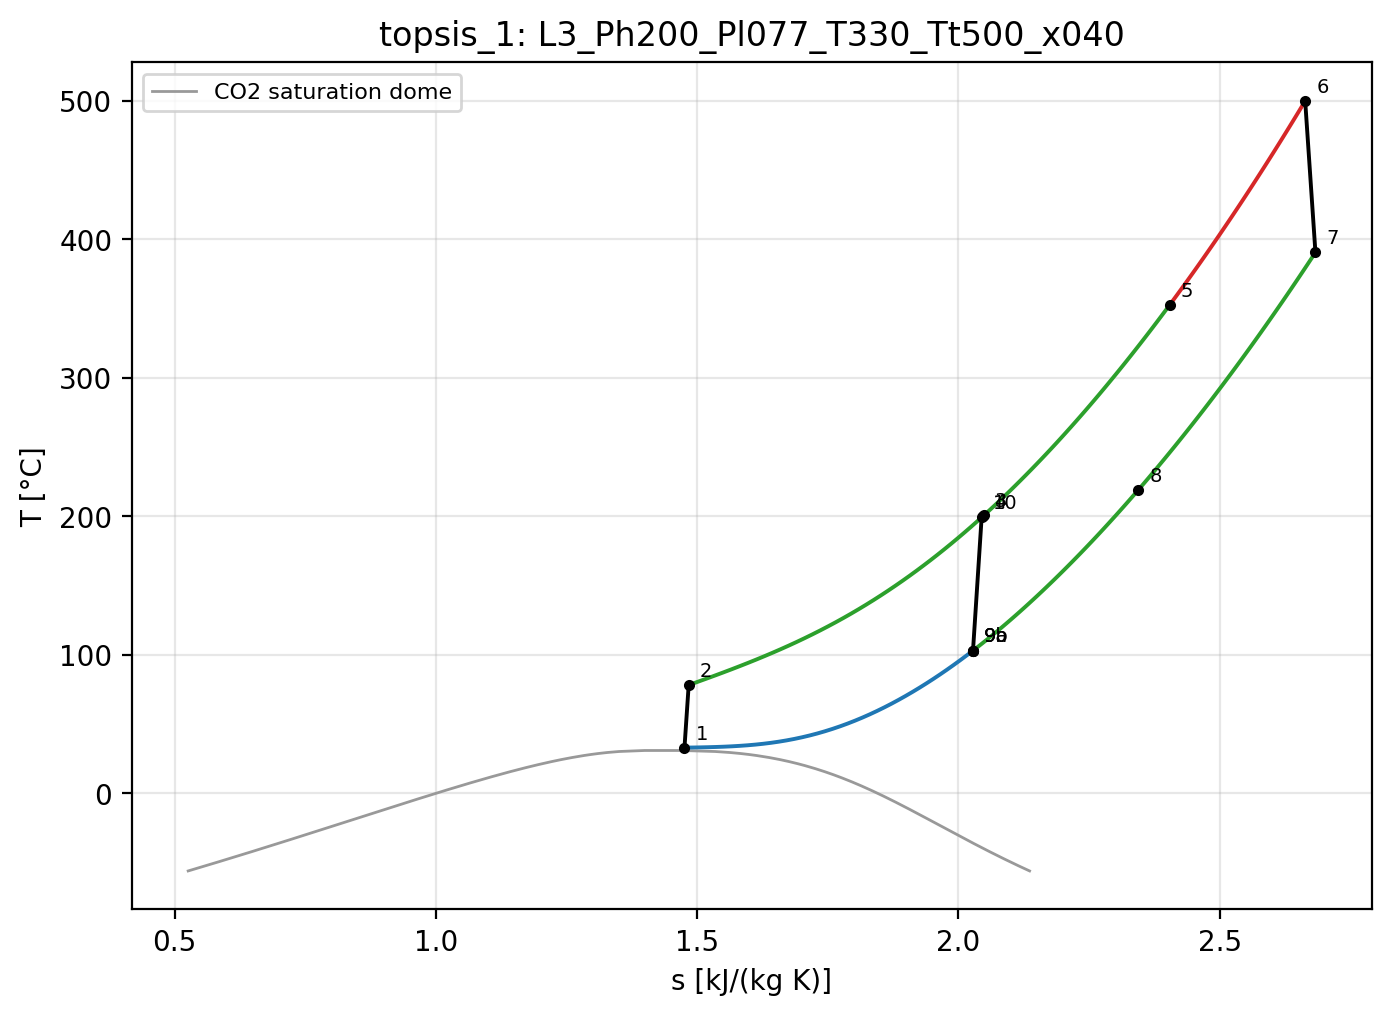
\includegraphics[width=0.49\textwidth]{figs/ts_selected.png}\hfill
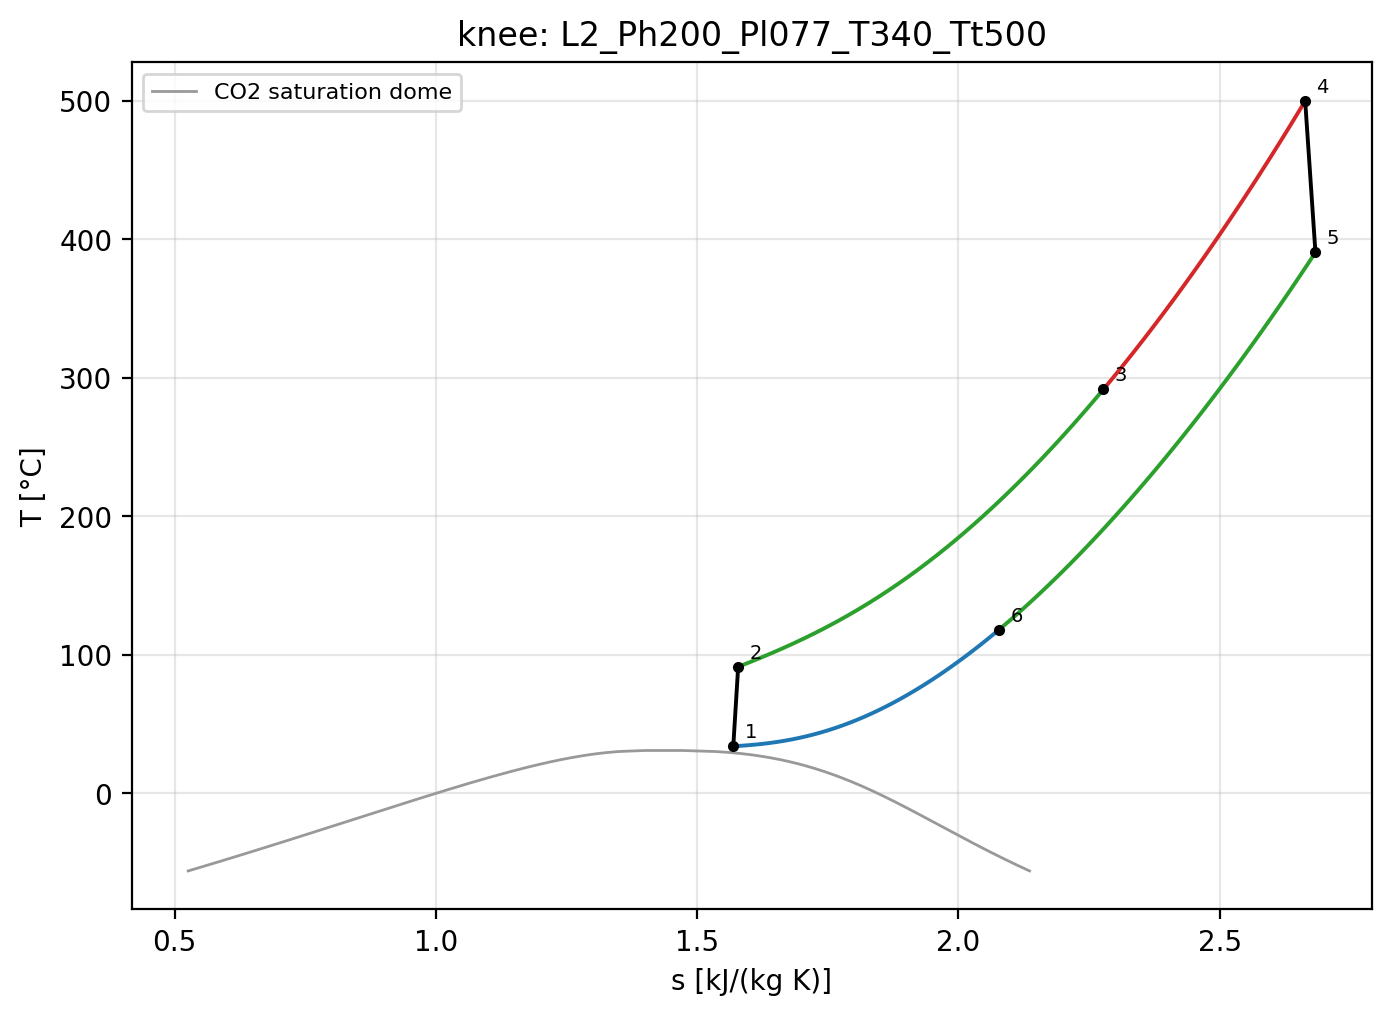
\includegraphics[width=0.49\textwidth]{figs/ts_baseline.png}
\caption{$T$--$s$ diagrams of the selected recompression design (left) and the layout~2 reference (right).}\label{fig:ts}
\end{figure}

The compressor inlet is \SI{2.0}{K} and \SI{0.32}{MPa} above the critical point (\SI{30.98}{\celsius}, \SI{7.377}{MPa}). The turbine inlet pressure and temperature and the compressor inlet pressure are at their limits. The inlet temperature and the split fraction are not. Raising the inlet from \SI{32}{\celsius} to \SI{33}{\celsius} costs 1.3 points of efficiency at the same split, but the cooler then rejects heat at a larger temperature difference, the cooling-water flow halves (\SI{638}{kg/s} against \SI{1282}{kg/s}), and the exchangers are \SI{3.1}{t} lighter.

\code{\path{core/export_states.py}, \path{data/shortlist.csv}, \path{data/states.csv}, \path{out/Top_N_topsis/}}

\subsection{What is given up}
\begin{itemize}
  \item \textbf{Against the highest-payout design} (layout~3, \SI{32}{\celsius}, $x = 0.36$; 42.3\%, \SI{78.2}{t}, \$187.7M): the selected design gives up 2.1 points of efficiency and \$8.8M of payout (4.7\%), and saves \SI{6.7}{t} (8.6\%).
  \item \textbf{Against the most efficient design} (layout~5; 42.5\%, \SI{86.5}{t}, \$186.4M): it gives up 2.3 points of efficiency and \$7.5M of payout, and is \SI{15.0}{t} lighter with one fewer compressor and one fewer cooler.
  \item \textbf{Against the layout~2 reference} (33.3\%, \SI{60}{t}, \$148.2M): it is \SI{11.5}{t} heavier, which costs \$2.9M, and its extra output is worth \$3.4M per year. The incremental payback is about 10 months (Table~\ref{tab:increment}), and the ten-year payout is \$30.7M higher.
  \item \textbf{Against the simple cycle} (layout~1, \SI{48.7}{t}, \$60.4M, outside the ranking): it is \SI{23}{t} heavier and earns about three times the payout.
\end{itemize}

\paragraph{Comparison with the baseline, step by step.} Table~\ref{tab:increment} repeats the given worked comparison with the computed values of the recuperated reference and the selected design. All values are per year of operation at \SI{7000}{h}. The payback in the last row is the incremental payback of Section~\ref{sec:objective}: it compares the added hardware with the added output only.

\begin{table}[h]\centering\small
\begin{tabular}{@{}r l l l@{}}
\toprule
 & Quantity & Calculation & Value\\
\midrule
1 & Reference net power & $0.3331 \times 100$ & \SI{33.31}{MWe}\\
2 & Reference heat per MWe & $100/33.31$ & \SI{3.00}{MWth/MWe}\\
3 & Candidate net power & $0.4017 \times 100$ & \SI{40.17}{MWe} (\SI{2.49}{MWth/MWe})\\
4 & Extra output & $40.17 - 33.31$ & \SI{6.86}{MWe}\\
5 & Extra annual energy & $6.86 \times 7000$ & \SI{48030}{MWh}\\
6 & Extra annual value & $48030 \times 70$ & \$3.36M per year\\
7 & Added mass & $71.52 - 60.00$ & \SI{11.52}{t}\\
8 & Added hardware cost & $11520 \times 250$ & \$2.88M\\
9 & Compactness & $33.31/60.00$ against $40.17/71.52$ & 0.555 against \SI{0.562}{MWe/t}\\
10 & Second-law efficiency & $\eta/\eta_\mathrm{Carnot}$ & 0.553 against 0.665\\
11 & Incremental payback & $2.88/3.36$ & 0.86 years (about 10 months)\\
\bottomrule
\end{tabular}
\caption{Selected design against the recuperated reference, following the given worked comparison.}\label{tab:increment}
\end{table}

The selected design is more compact than the reference in MWe per tonne as well as more efficient: the extra exchanger mass is more than matched by the extra output. Under the omissions listed in Section~\ref{sec:limits}, the added hardware is recovered within the first year of operation.

\code{\path{data/results_econ.csv}, \path{out/summary.md}}

\subsection{Sensitivity}
We test whether the selection survives changes in two things: the lifetime $N$ and the grid spacing.

\paragraph{Lifetime $N$: the selection holds.} The payout weighs efficiency against hardware, $\Pi_N = N\,\eta\,\dot Q_\mathrm{th}\,t_\mathrm{op}\,c_e - c_m\,m$. A larger $N$ gives efficiency more weight and favours heavier, more efficient designs; a smaller $N$ favours light ones. We repeated the ranking for $N$ = 5, 10 and 20 years (Table~\ref{tab:life}). The knee and TOPSIS pick the same design at all three, and the highest-payout design does not change either. The recommendation therefore does not hinge on the choice of ten years.

\begin{table}[h]\centering\small
\setlength{\tabcolsep}{4pt}\begin{tabular}{@{}clll@{}}
\toprule
$N$ (years) & Knee & TOPSIS first & Highest payout\\
\midrule
5 & L3, \SI{33}{\celsius}, $x = 0.40$ (\$80.5M) & L3, \SI{33}{\celsius}, $x = 0.40$ (\$80.5M) & L3, \SI{32}{\celsius}, $x = 0.36$ (\$84.1M)\\
10 & L3, \SI{33}{\celsius}, $x = 0.40$ (\$178.9M) & L3, \SI{33}{\celsius}, $x = 0.40$ (\$178.9M) & L3, \SI{32}{\celsius}, $x = 0.36$ (\$187.7M)\\
20 & L3, \SI{33}{\celsius}, $x = 0.40$ (\$375.8M) & L3, \SI{33}{\celsius}, $x = 0.40$ (\$375.8M) & L3, \SI{32}{\celsius}, $x = 0.36$ (\$395.0M)\\
\bottomrule
\end{tabular}
\caption{Sensitivity to the lifetime $N$, layouts 2 to 6. L3 is layout 3.}\label{tab:life}
\end{table}

\paragraph{Grid spacing: partly stable.} In the first sweep, with inlet temperatures of 32, 36 and \SI{40}{\celsius} and a split step of 0.05, TOPSIS picked layout~3 at \SI{20}{MPa} and \SI{7.7}{MPa}, \SI{32}{\celsius} and $x = 0.40$. After the refinement, with inlet temperatures of 32, 33 and \SI{34}{\celsius} and a split step of 0.01, it picked the same layout and pressures at \SI{33}{\celsius} and $x = 0.40$. The layout and pressures never moved, so they are firm. The inlet temperature moved by one grid step, so it is known only to about the grid spacing.

\code{\path{core/summary.py}}

\subsection{Cautions on the selected design}
\paragraph{The optimum split may lie just past the grid.} The refined split range ends at 0.40, and the TOPSIS score is still rising there (Table~\ref{tab:splitedge}). When the best point sits on the boundary of the search and the trend is still upward, the true optimum is probably a little beyond it, perhaps at 0.41 to 0.43. The gains shrink with each step, so it is unlikely to be far. This is why we state the split only to about 0.02 and the inlet temperature to about \SI{1}{K}, the refined grid step.

\begin{table}[h]\centering\small
\begin{tabular}{@{}lcccccc@{}}
\toprule
Split fraction $x$ & 0.35 & 0.36 & 0.37 & 0.38 & 0.39 & 0.40\\
\midrule
TOPSIS score & 0.796 & 0.803 & 0.808 & 0.813 & 0.816 & 0.818\\
\bottomrule
\end{tabular}
\caption{TOPSIS score against split fraction for layout~3 at \SI{20}{MPa}, \SI{7.7}{MPa} and \SI{33}{\celsius}.}\label{tab:splitedge}
\end{table}

\paragraph{The inlet sits at the steepest part of the \cotwo{} property curve.} The critical point of \cotwo{} is \SI{30.98}{\celsius} and \SI{7.38}{MPa}. At \SI{7.7}{MPa}, just above the critical pressure, \cotwo{} changes from liquid-like to gas-like over a narrow band of temperature, and the selected inlet lies inside that band (Table~\ref{tab:inletprops}). At \SI{33}{\celsius} the specific heat is almost exactly at its peak. A drift of \SI{1}{K} either way changes the density by more than 20\%, which changes the work and flow of the compressor substantially. In a real plant the inlet temperature wanders with the cooling-water temperature, the load and the control system. This study computes one steady design point and does not examine how the cycle behaves when the inlet drifts (off-design or transient operation). The computed efficiency therefore assumes that the inlet is held tightly at \SI{33}{\celsius}, which we have not shown to be achievable.

\begin{table}[h]\centering\small
\begin{tabular}{@{}lcccc@{}}
\toprule
Inlet temperature (\si{\celsius}) & 32 & \textbf{33} & 34 & 36\\
\midrule
Density (\si{kg/m^3}) & 602 & \textbf{431} & 338 & 289\\
$c_p$ (\si{kJ/kg.K}) & 15.1 & \textbf{65.5} & 14.9 & 6.8\\
\bottomrule
\end{tabular}
\caption{\cotwo{} properties at \SI{7.7}{MPa} near the selected compressor inlet temperature (CoolProp).}\label{tab:inletprops}
\end{table}

\section{Recommendation}
The recommended cycle is the \textbf{recompression cycle (layout 3)} at \SI{20}{MPa} turbine inlet pressure, \SI{7.7}{MPa} and \SI{33}{\celsius} compressor inlet, \SI{500}{\celsius} turbine inlet and a split fraction of 0.40. It delivers \SI{40.2}{MWe} at 40.2\% efficiency, has a mass of \SI{71.5}{t}, and returns \$178.9M over ten years.

The reasons are:
\begin{enumerate}
  \item It is the knee of the Pareto front and is ranked first by TOPSIS, and both hold for every lifetime tested.
  \item Against the recuperated baseline it adds 6.9 points of efficiency for \SI{11.5}{t} of extra hardware, and the added output recovers the added hardware cost in about 10 months (incremental payback, Table~\ref{tab:increment}).
  \item It needs one extra compressor and one extra recuperator. Layouts 5 and 6 need a second extra compressor and a second cooler, and no design of either is on the Pareto front except one light layout~6 design with a lower payout.
  \item Intercooling is not recommended in either form. It adds mass without a matching gain in efficiency.
\end{enumerate}

The choice depends on how much mass matters. Payout already includes the cost of hardware, so if mass has no value beyond its cost, the best design is the same cycle at \SI{32}{\celsius} and $x = 0.36$: 42.3\%, \SI{78.2}{t} and \$187.7M. The recommended design gives up \$8.8M (4.7\%) of that payout to be \SI{6.7}{t} (8.6\%) lighter and to need half the cooling water. If mass were a hard limit near \SI{60}{t}, the recuperated cycle at \SI{20}{MPa} and \SI{34}{\celsius} would be the choice, at a cost of \$30.7M of payout over ten years.

Two cautions apply (Section~\ref{sec:results}, \emph{Cautions on the selected design}). The selected split is on the edge of the refined grid, where the score is still rising, so the best split may be slightly above 0.40. And the inlet at \SI{33}{\celsius} and \SI{7.7}{MPa} sits at the peak of the \cotwo{} specific heat, where a \SI{1}{K} drift changes the density by more than 20\%; the design's performance depends on holding that inlet state, which this steady-state study does not test.


\appendix
\section{Numerical methods}\label{app:numerics}

\subsection{Solver structure}
The cycle solver is written in Python. A layout is a list of components and the streams that connect them, with no numbers in it. A case adds the numbers: pressure levels, temperatures, efficiencies and exchanger specifications. Solving a case takes four steps:
\begin{enumerate}
  \item \textbf{Pressures.} Every stream pressure is found by direct propagation from the fixed pressure levels through the components. No iteration is needed.
  \item \textbf{Flow fractions.} The fraction of the total flow in every stream is found from the splitter settings.
  \item \textbf{Order of evaluation.} The components are ordered so that each is evaluated after its inlets are known. Where the layout has a loop (layouts~3, 5 and~6), one stream is chosen as a guess.
  \item \textbf{Evaluation.} Components are evaluated in order. With a guessed stream, the pass is repeated by successive substitution until the guessed enthalpy changes by less than $10^{-8}$ (relative).
\end{enumerate}
Layouts~1, 2 and~4 need no iteration. A design that fails to converge, or that violates a physical check (a temperature cross in an exchanger, a failed energy balance), is flagged and recorded as infeasible. It does not stop the sweep.

\code{\path{cycles/solve.py}, \path{cycles/passes/}}

\subsection{Properties}
All fluid properties come from CoolProp~\cite{coolprop}, for both fluids in the model: \cotwo{} on the cycle side (Span--Wagner equation of state~\cite{spanwagner}) and water on the cooler side (IAPWS-95 formulation~\cite{iapws}). Pressure and enthalpy are the independent pair for every stream. Pressure and temperature are used where a temperature is specified (turbine inlet, cooler outlet, water inlet), and pressure and entropy for the isentropic outlet state of a compressor or turbine. No ideal-gas or constant-$c_p$ relation is used anywhere in the cycle model.

\code{\path{cycles/properties/coolprop.py}}

\subsection{Recuperator: effectiveness, pinch and conductance}
The recuperator calculation is the core of the model, because near the critical point the specific heats of the two streams differ strongly and change along the exchanger. Textbook methods that assume constant $c_p$ (a single log-mean temperature difference, or effectiveness--NTU charts) do not apply. The calculation is done in five steps, all in terms of enthalpy.

\paragraph{1. Maximum possible duty.} For a counterflow exchanger two limits apply: the hot stream cannot leave colder than the cold stream enters, and the cold stream cannot leave hotter than the hot stream enters. In enthalpy, with $\dot m_h$ and $\dot m_c$ the flows on the two sides,
\begin{equation}
\dot Q_\mathrm{max} = \min\Big[\;\dot m_h\big(h_{h,\mathrm{in}} - h(P_h, T_{c,\mathrm{in}})\big),\;\; \dot m_c\big(h(P_c, T_{h,\mathrm{in}}) - h_{c,\mathrm{in}}\big)\;\Big].
\end{equation}
Each term needs one CoolProp call at the other stream's inlet temperature. Which limit is smaller is a result of the calculation and is not assumed. In the recompression cycle the two sides of the low-temperature recuperator also carry different flows, $\dot m_c = (1-x)\dot m_h$, and this enters both terms.

\paragraph{2. Duty and outlet states.} With the effectiveness fixed at $\varepsilon = 0.90$,
\begin{equation}
\dot Q = \varepsilon\, \dot Q_\mathrm{max}, \qquad h_{h,\mathrm{out}} = h_{h,\mathrm{in}} - \frac{\dot Q}{\dot m_h}, \qquad h_{c,\mathrm{out}} = h_{c,\mathrm{in}} + \frac{\dot Q}{\dot m_c}.
\end{equation}
The outlets follow directly from the energy balance, so the recuperator itself needs no iteration. Effectiveness defined this way, on enthalpy, stays meaningful when $c_p$ varies; one defined on temperature would not.

\paragraph{3. Temperature profile.} A fixed effectiveness does not guarantee that the two streams stay apart inside the exchanger. Because $c_p$ varies, the temperature curves are not straight, and they can come closest, or even cross, somewhere in the middle rather than at an end. To find out, the duty is divided into $N = 100$ equal slices, and the enthalpies at the $N+1$ boundaries, counted from the cold end, are
\begin{equation}
h_{c,j} = h_{c,\mathrm{in}} + \frac{j}{N}\,\frac{\dot Q}{\dot m_c}, \qquad h_{h,j} = h_{h,\mathrm{out}} + \frac{j}{N}\,\frac{\dot Q}{\dot m_h}, \qquad j = 0, 1, \dots, N.
\end{equation}
These are exact from the energy balance. Temperatures follow from $T_{c,j} = T(P_c, h_{c,j})$ and $T_{h,j} = T(P_h, h_{h,j})$ through CoolProp, and the local difference is $\Delta T_j = T_{h,j} - T_{c,j}$. Dividing in duty rather than in length means no geometry is needed.

\paragraph{4. Pinch and feasibility.} The pinch is the smallest local difference,
\begin{equation}
\Delta T_\mathrm{pinch} = \min_j \Delta T_j .
\end{equation}
If $\Delta T_\mathrm{pinch} \le 0$ the curves cross, the specified duty is physically impossible, and the design is recorded as not solved. If $0 < \Delta T_\mathrm{pinch} < \SI{5}{K}$ the design is solved but rejected as infeasible. This is the check that removes most infeasible designs (Table~\ref{tab:grid}): towards the cold end of a recuperator the high-pressure stream's $c_p$ rises steeply as it approaches the pseudo-critical temperature, and the pinch moves inside the exchanger.

\paragraph{5. Conductance.} A single log-mean temperature difference is exact only when $\Delta T$ varies linearly with duty, which needs constant $c_p$. Each slice is short enough to be treated that way, so the conductance is the sum over slices:
\begin{equation}
UA = \sum_{j=1}^{N} \frac{\dot Q/N}{\Delta T_{\mathrm{lm},j}}, \qquad \Delta T_{\mathrm{lm},j} = \frac{\Delta T_j - \Delta T_{j-1}}{\ln(\Delta T_j/\Delta T_{j-1})}.
\end{equation}
If the two end differences of a slice are equal to within $10^{-9}$ relative, their arithmetic mean replaces the log-mean. $UA$ then gives the recuperator mass through $k_{UA}$ (Section~\ref{sec:objective}).

\paragraph{Scaling with mass flow.} Inside the solver every flow is a fraction of the total cycle flow, so $\dot Q$ and $UA$ are first obtained per kilogram per second of total flow. The total flow is known only after the cycle is solved, from the fixed heater duty, $\dot m = \dot Q_\mathrm{th}/(h_\mathrm{turb,in} - h_\mathrm{heater,in})$, and $UA$ is then multiplied by $\dot m$ to give \si{kW/K}.

\paragraph{Accuracy.} Enthalpies at the nodes are exact, so the only discretisation error lies in locating the pinch between nodes and in the log-mean within each slice. Appendix~\ref{app:validation} shows that $N = 100$ and $N = 1000$ agree to better than 0.01\%.

\code{\path{cycles/blocks/heat_exchanger.py}, \path{cycles/physics/hx_limits.py}, \path{cycles/physics/hx_profile.py}, \path{cycles/physics/hx_sizing.py}}

\subsection{Cooler: water flow from the pinch, then conductance}
A cooler is a counterflow heat exchanger with \cotwo{} on the hot side and cooling water on the cold side, so it uses the same profile and conductance routines as the recuperator. Water properties come from CoolProp (IAPWS-95). The water enters at \SI{25}{\celsius} and is held at \SI{6}{bar}. What differs from the recuperator is which quantities are known and which are found.

\paragraph{Duty: fixed by the cycle.} The cooler must bring the \cotwo{} to the compressor inlet temperature, so its outlet state $h(P, \Tin)$ is fixed and so is its duty,
\begin{equation}
\dot Q_\mathrm{cooler} = \dot m_\mathrm{CO_2}\big(h_\mathrm{CO_2,in} - h(P, \Tin)\big).
\end{equation}

\paragraph{Water flow: found from the pinch.} The water flow $\dot m_w$ is not given, and it decides everything else. For a trial flow the water outlet enthalpy follows from the energy balance, $h_{w,\mathrm{out}} = h_{w,\mathrm{in}} + \dot Q_\mathrm{cooler}/\dot m_w$. The same equal-duty profile is then built, with water as the cold stream, and its pinch found as in step~4 of the recuperator. Less water heats up more and approaches the \cotwo{} temperature, so the pinch shrinks; more water stays cool and the pinch grows. The pinch therefore rises steadily with $\dot m_w$, and the flow that gives the decided pinch of \SI{5}{K} is the root of
\begin{equation}
f(\dot m_w) = \Delta T_\mathrm{pinch}(\dot m_w) - \SI{5}{K} = 0 .
\end{equation}
It is found by bisection:
\begin{itemize}
  \item \textbf{Lower bound:} the flow at which the water would leave \SI{0.01}{K} below the \cotwo{} inlet temperature (least water; pinch near zero).
  \item \textbf{Upper bound:} the flow at which the water warms by only \SI{0.5}{K} (most water).
  \item \textbf{Stopping rule:} bracket width below $10^{-6}$ relative.
\end{itemize}
With the \cotwo{} leaving at \SI{32}{\celsius} or more against \SI{25}{\celsius} water, the temperature difference at the cold end is at least \SI{7}{K}, so a \SI{5}{K} pinch can always be reached. As a guard, a design whose computed cooler pinch differs from \SI{5}{K} by more than \SI{0.01}{K} is rejected.

\paragraph{Conductance: from the final profile.} With the water flow known, the profile is built once more and the cooler $UA$ is summed slice by slice exactly as for the recuperator. The cooler mass then follows from the same $k_{UA}$. The water flow itself is reported, because cooling-water demand matters for siting a reactor.

\paragraph{Cost and resolution.} Every trial of the bisection builds a full profile, which makes the cooler the most expensive step of a solve (about 95\% of the time). The sweeps use 50 slices; the shortlisted designs are re-solved with 100, and the cooler $UA$ at 50 slices is within 0.05\% of the 100-slice value.

\paragraph{The simple-cycle failure.} The \SI{6}{bar} water pressure explains why half of the simple-cycle designs did not solve (Section~\ref{sec:results}). Without a recuperator the cooler receives turbine exhaust at about \SI{400}{\celsius}. The lower bound of the bisection then asks for water leaving close to that temperature, above the boiling point of water at \SI{6}{bar} (\SI{159}{\celsius}), where CoolProp cannot return a liquid state. The same machinery works for every other layout, where the cooler inlet is far cooler.

\code{\path{cycles/blocks/cooler.py}, \path{cycles/physics/coolant.py}, \path{cycles/numerics/roots.py}}

\subsection{Sweep and bookkeeping}
Each design point has an identifier that encodes its layout and operating variables as integers, for example \texttt{L3\_Ph200\_Pl077\_T320\_Tt500\_x030} for layout~3 at $\Ph = \SI{20.0}{MPa}$, $\Pl = \SI{7.7}{MPa}$, $\Tin = \SI{32.0}{\celsius}$, $\Tt = \SI{500}{\celsius}$ and $x = 0.30$. The calculation runs as a chain of files: the grid of inputs, the solver output (efficiency, conductances and pinches of feasible points, with a separate list of infeasible points and the reason for each), and the economic results (mass, cost, payout and rankings). Economic assumptions can therefore be changed without solving any cycle again. The grid for each layout is given in Table~\ref{tab:grid}.

\code{\path{helpers/ids.py}, \path{core/make_inputs.py}, \path{core/solve_points.py}}

\section{Validation}\label{app:validation}

\subsection{Against a closed-form solution}
With an ideal-gas property model in place of CoolProp, the solver reproduces the air-standard Brayton cycle formulas for efficiency, net work, heat input and back-work ratio to within the test tolerance of $10^{-4}$ (relative). This checks the cycle algebra independently of the \cotwo{} properties.

\code{\path{tests/test_solver.py}}

\subsection{Against published \scotwo{} work}
\begin{table}[!htbp]\centering\small
\begin{tabular}{llll}
\toprule
Check & Reference & Published & This solver\\
\midrule
State table, enthalpy (worst error) & Dostal~\cite{dostal}, Table 10.2 & -- & 0.0015\%\\
State table, entropy (worst error) & Dostal & -- & 0.39\%\\
Compressor outlet, $\eta_c = 0.89$ & Dostal & \SI{327.26}{kJ/kg} & \SI{327.26}{kJ/kg}\\
Turbine outlet, $\eta_t = 0.90$ & Dostal & \SI{914.45}{kJ/kg} & \SI{914.46}{kJ/kg}\\
Recompression cycle efficiency & Kim et al.~\cite{kim} & 44.67\% & 44.669\%\\
Optimum split fraction & Kim et al. & 0.307 & 0.307\\
Optimum pressure ratio & Kim et al. & 2.6 & 2.6\\
\bottomrule
\end{tabular}
\caption{Comparison with published values. The two optima were found by sweeping around the published value and confirming that the maximum falls on it.}
\end{table}

\code{\path{tests/test_solver.py}}

\subsection{Independent recalculation of one design}
The recuperated cycle at $\Ph = \SI{20}{MPa}$, $\Pl = \SI{7.7}{MPa}$, $\Tin = \SI{32}{\celsius}$, $\Tt = \SI{500}{\celsius}$ was recomputed in a separate short script that uses only CoolProp property calls and none of the solver's code, with 1000 slices per exchanger. Table~\ref{tab:indep} compares the two and Table~\ref{tab:states} gives the state points.

\begin{table}[!htbp]\centering\small
\begin{tabular}{lrr}
\toprule
Quantity & Solver ($N=100$) & Independent ($N=1000$)\\
\midrule
Thermal efficiency & 0.3271985 & 0.3271985\\
Mass flow (\si{kg/s}) & 341.48 & 341.48\\
Recuperator $UA$ (\si{kW/K}) & 1669.53 & 1669.56\\
Recuperator pinch (\si{K}) & 25.14 & 25.14\\
Cooler $UA$ (\si{kW/K}) & 7692.51 & 7693.14\\
Cooler pinch (\si{K}) & 5.000 & 5.000\\
\bottomrule
\end{tabular}
\caption{Solver against an independent recalculation.}\label{tab:indep}
\end{table}

\begin{table}[!htbp]\centering\small
\begin{tabular}{clrrrr}
\toprule
State & Location & $P$ (\si{MPa}) & $T$ (\si{\celsius}) & $h$ (\si{kJ/kg}) & $s$ (\si{kJ/kg.K})\\
\midrule
1 & Compressor inlet & 7.7 & 32.00 & 306.23 & 1.3463\\
2 & Compressor outlet & 20.0 & 60.90 & 326.75 & 1.3531\\
3 & Heater inlet & 20.0 & 262.63 & 680.45 & 2.2107\\
4 & Turbine inlet & 20.0 & 500.00 & 973.29 & 2.6636\\
5 & Turbine outlet & 7.7 & 390.60 & 856.95 & 2.6832\\
6 & Cooler inlet & 7.7 & 86.04 & 503.26 & 1.9655\\
\bottomrule
\end{tabular}
\caption{State points of the recalculated design (layout~2 numbering).}\label{tab:states}
\end{table}

From these states: compressor work \SI{20.52}{kJ/kg}, turbine work \SI{116.34}{kJ/kg}, heat input \SI{292.84}{kJ/kg}, so $\eta = (116.34 - 20.52)/292.84 = 0.3272$. In the recuperator the hot-side limit binds (\SI{393.0}{kJ/kg} against \SI{512.3}{kJ/kg} for the cold side), which is the heat-capacity mismatch of Section~2 in numbers. The cooler rejects \SI{67.3}{MW} to \SI{1397}{kg/s} of water, which leaves at \SI{36.5}{\celsius}.

\code{\path{independent_check.py} (supplied with this report)}

\section{Modelling decisions}\label{app:decisions}

Table~\ref{tab:decisions} records each point where the given data left a choice open, what we chose and why.

\begin{table}[!htbp]\centering\small
\begin{tabularx}{\textwidth}{>{\raggedright\arraybackslash}p{3.3cm}>{\raggedright\arraybackslash}p{4.2cm}X}
\toprule
Question & Decision & Reason\\
\midrule
What sets the pressure ratio? & $\Ph$ is fixed at the compressor outlet and $\Pl$ at its inlet. The ratio is a result. & The compressor is the only component that raises pressure, so its outlet is the highest pressure in the cycle. The \SI{20}{MPa} limit must apply there.\\
Recuperator: fix effectiveness or pinch? & Effectiveness 0.90. Reject designs with pinch below \SI{5}{K}. & 0.90 is given as the baseline and \SI{5}{K} as a minimum. Both are honoured without tuning each design.\\
How is the cooler sized? & Minimum \cotwo--water difference of \SI{5}{K}. & Only the water temperature is given. A pinch rule fixes the water flow, and the flow fixes $UA$, with nothing left to guess.\\
Cooler mass & \SI{2.5}{kg} per \si{kW/K}, as for recuperators. & No figure is given for coolers. The same exchanger technology is assumed.\\
Baseline mass split & $M_0$ calibrated at the most efficient feasible recuperated design. & \SI{60}{t} is given for the baseline layout. Calibrating once lets every other design be measured against it on the same basis.\\
Is the given 10~t recuperator figure used? & No. & It appears only inside a worked example. Exchanger masses are computed from $UA$ here.\\
Cost model & Cost $= \SI{250}{US\$/kg} \times$ mass. & A single price is given for installed hardware.\\
Economic measure & Net return over $N = 10$ years. & It puts a one-time cost and a yearly income on one scale, and needs no reference design.\\
Objectives & Lifetime payout and mass. & Payout combines efficiency and cost. Mass represents compactness. The critical-point margin is treated as a constraint and reported.\\
Carnot efficiency & Computed per design from $\Tin$ and $\Tt$. & Both temperatures are swept, so a single constant would misstate the second-law efficiency.\\
Turbine inlet temperature & Swept at and below \SI{500}{\celsius}. & It is given as an upper limit.\\
Is the simple cycle ranked? & No. It is solved and reported, but left out of the Pareto front, knee and TOPSIS. & At 15\% efficiency it is not a candidate, but as the lightest layout it would set the light end of the front and move the knee towards light designs.\\
What is layout 5? & Layout 3 with two intercooled main-compression stages. & The layout is given only as recompression with intercooling. The recompressor takes warm fluid, so intercooling is applied to the main compressor only.\\
\SI{7.7}{MPa} limit in layout 6 & Applied to the main compressor inlet only; the pre-compressor inlet ($\Pe$) is below it. & The layout requires $\Pe$ below the main compressor inlet pressure. The inlet stays single-phase, since its temperature is above the critical temperature.\\
The literal reading of that limit & Also ranked (strict ranking), but not followed. & It decides the result, so its outcome is reported beside ours.\\
When to stop refining & When the winners stop moving and none lies on a free edge of its range. & Further points in the same ranges would not change the answer.\\
$M_0$ in the studies & Recalibrated on the same reference design when the cycle model changes (S1); held at \SI{39.06}{t} where recalibration would switch the reference design (S3). & $M_0$ stands for the hardware outside the exchangers, which a change of reference design does not alter. A constant shift of every mass leaves the Pareto front and knee unchanged but moves TOPSIS, which scales by vector length.\\
\bottomrule
\end{tabularx}
\caption{Modelling decisions.}\label{tab:decisions}
\end{table}

\section{Code and repository}\label{app:code}

All code, input grids, result tables and plots of this study are in the repository
\begin{center}
\url{https://github.com/scp15156402/SMR_sCO2_Optimiser}
\end{center}
This report corresponds to branch \path{main} at tag \path{final}. Earlier states are kept as tags: \path{rebuild} is the version submitted for the course, and \path{extended-v1} is the converged refinement before the extended studies. The compiled report is \path{Full_Report.pdf} at the top of the repository, and its \LaTeX{} source is in \path{Documents/Final Report/}. The code is Python and uses CoolProp for properties.

\subsection{Folder structure}
{\small
\begin{verbatim}
config.py            given values, constraints, decided values, calibrated M0
grids.py             sweep ranges for each layout
cycles/              general cycle solver (knows nothing about CO2 or Brayton)
  stream.py            a stream: fluid, P, h, flow fraction
  flowsheet.py         a layout: list of blocks and the streams between them
  case.py, specs.py    one run: fluid, size, boundary state, block parameters
  solve.py             runs the passes and returns the result
  passes/              pressure, flow, ordering, tear
  blocks/              compressor, turbine, heater, cooler, heat_exchanger,
                       splitter, mixer
  physics/             isentropic step, exchanger profile, pinch, UA,
                       coolant sizing, mixing
  properties/          CoolProp and ideal-gas property back ends
  numerics/            bisection and secant root finders
brayton_cycle/       the six layouts, written as data
  simple.py, recuperated.py, recompression.py, intercooled.py,
  recomp_intercooled.py, partial_cooling.py
helpers/
  ids.py               design identifier <-> operating variables
  builders.py          identifier -> solver case, for each layout
  checks.py            feasibility checks and the two-stage evaluation
  ranking.py           Pareto front, knee, TOPSIS
core/                the pipeline, run in this order
  make_inputs.py       grids.py -> data/inputs.csv
  solve_points.py      inputs -> data/results_raw.csv, data/infeasible.csv
  calibrate.py         layout 2 reference -> M0
  economics.py         mass, cost, payout, ranking -> data/results_econ.csv
                       (and the strict ranking -> data/results_econ_strict.csv)
  export_states.py     shortlisted designs -> data/states.csv, shortlist.csv
  plots.py             figures and T-s diagrams -> out/
  summary.py           out/summary.md
  refine.py            refinement rounds until convergence -> out/convergence.md
  studies/             extended studies S1-S9 -> out/studies/
data/                input and result tables (CSV)
out/                 plots, T-s diagrams, summary
tests/               tests of the solver, identifiers, checks, ranking, layouts
\end{verbatim}}

\subsection{Solver approach}
The solver in \path{cycles/} is built in layers, and each layer uses only the ones below it: properties and root finders, then physics functions, then blocks, then passes, then \path{solve.py}.

\paragraph{Streams.} A stream stores the fluid, pressure, specific enthalpy and its fraction of the total mass flow. Temperature, entropy and density are computed from $(P, h)$ when needed. Pressure and enthalpy are used because they identify a state everywhere, including close to the critical point where properties change steeply with temperature.

\paragraph{Blocks.} Each component type is one module in \path{cycles/blocks/}. A block declares its inlet and outlet ports, how it relates the pressures of its ports, how it relates their flows, and an \texttt{evaluate} function that returns the outlet streams from the inlet streams. The seven blocks are compressor, turbine, heater, cooler, two-stream heat exchanger, splitter and mixer. The component equations are those of Section~\ref{sec:model}.

\paragraph{Layouts as data.} A layout is not code. It is a list of blocks with named streams between them. The recompression cycle, for example, is written in \path{brayton_cycle/recompression.py} as
{\small
\begin{verbatim}
Node("MC",    "compressor",     {"in": "s1"},  {"out": "s2"}),
Node("LTR",   "heat_exchanger", {"cold_in": "s2", "hot_in": "s8"},
                                {"cold_out": "s3", "hot_out": "s9"}),
Node("SPLIT", "splitter",       {"in": "s9"},  {"out": ["s9a", "s9b"]}),
Node("PC",    "cooler",         {"in": "s9a"}, {"out": "s1"}),
Node("RC",    "compressor",     {"in": "s9b"}, {"out": "s10"}),
Node("MIX",   "mixer",          {"in": ["s3", "s10"]}, {"out": "s4"}),
Node("HTR",   "heat_exchanger", {"cold_in": "s4", "hot_in": "s7"},
                                {"cold_out": "s5", "hot_out": "s8"}),
Node("HEATER","heater",         {"in": "s5"},  {"out": "s6"}),
Node("TURB",  "turbine",        {"in": "s6"},  {"out": "s7"}),
\end{verbatim}}
\noindent Adding a layout therefore means writing one such list and one entry in \path{helpers/builders.py} that supplies its numbers. We added layout~5 this way without changing the solver.

\paragraph{Passes.} \path{solve.py} runs four passes over a layout (Appendix~\ref{app:numerics}): the pressure pass fixes every stream pressure, the flow pass fixes every flow fraction, the ordering pass sorts the blocks so that each is evaluated after its inlets are known, and the tear pass handles loops. Layouts 3, 5 and 6 contain a loop through the recuperators. One stream in the loop is guessed, the blocks are evaluated in order, and the guess is replaced by the computed value until it stops changing.

\paragraph{Cases.} A case gives a layout its numbers: the fluid, the thermal power, the compressor inlet state, and the parameters of each block. \path{helpers/builders.py} builds the case for a design from its identifier and \path{config.py}, so no number is typed twice.

\paragraph{Two-stage evaluation.} \path{helpers/checks.py} first solves the cycle without the water side, which is fast, and applies the constraints. Only feasible designs are solved again with the cooling-water sizing, which takes about 95\% of the solve time.

\subsection{Where each part of the report is computed}
\begin{table}[h]\centering\small
\begin{tabularx}{\textwidth}{@{}l >{\raggedright\arraybackslash}X@{}}
\toprule
Report section & Files\\
\midrule
\ref{sec:layouts} Cycle layouts & \path{brayton_cycle/*.py}, \path{helpers/builders.py}\\
\ref{sec:model} Compressor and turbine & \path{cycles/blocks/compressor.py}, \path{turbine.py}, \path{cycles/physics/isentropic.py}\\
\ref{sec:model} Heater and mass flow & \path{cycles/blocks/heater.py}, \path{cycles/solve.py}\\
\ref{sec:recup} Recuperator & \path{cycles/blocks/heat_exchanger.py}, \path{cycles/physics/hx_limits.py}, \path{hx_profile.py}, \path{hx_sizing.py}\\
\ref{sec:cooler} Coolers & \path{cycles/blocks/cooler.py}, \path{cycles/physics/coolant.py}\\
\ref{sec:model} Pressures, splitting and mixing & \path{cycles/passes/pressure.py}, \path{flow.py}, \path{cycles/blocks/splitter.py}, \path{mixer.py}\\
\ref{sec:objective} Constraints & \path{config.py} (section B), \path{helpers/checks.py}\\
\ref{sec:objective} Mass, cost, payout & \path{core/calibrate.py}, \path{core/economics.py}\\
\ref{sec:objective} Selection & \path{helpers/ranking.py}\\
\ref{sec:objective} Fixed parameters & \path{config.py}\\
\ref{sec:results} Grid, refinement and feasible set & \path{grids.py}, \path{core/make_inputs.py}, \path{core/solve_points.py}, \path{core/refine.py}, \path{data/infeasible.csv}, \path{out/convergence.md}\\
\ref{sec:results} Strict ranking & \path{core/economics.py}, \path{data/results_econ_strict.csv}\\
\ref{sec:results} Calibration & \path{core/calibrate.py}\\
\ref{sec:results} Trends, Pareto front, $T$--$s$ diagrams & \path{core/plots.py}, \path{out/}\\
\ref{sec:results} Best designs, knee, TOPSIS, sensitivity & \path{core/economics.py}, \path{core/summary.py}, \path{out/summary.md}\\
\ref{sec:results} Selected design and its states & \path{core/export_states.py}, \path{data/states.csv}, \path{data/shortlist.csv}\\
\ref{sec:limits}, \ref{sec:studies} Extended studies S1--S9 & \path{core/studies/s1_*.py} to \path{s9_*.py}, \path{core/studies/run_all.py}, \path{out/studies/}\\
\ref{app:numerics} Numerical methods & \path{cycles/solve.py}, \path{cycles/passes/tear.py}, \path{cycles/numerics/roots.py}, \path{helpers/ids.py}\\
\ref{app:validation} Validation & \path{tests/test_solver.py} and the other files in \path{tests/}\\
\bottomrule
\end{tabularx}
\caption{Report sections and the files that compute them.}\label{tab:files}
\end{table}

\section{Authorship and use of AI}\label{app:contrib}

\paragraph{Course project.} The first version of this study was the ME~306 course project of a team of five: Siddhant Patil (24B2121), Vaishnavi Shivai (24B2116), Avinav Shekhar (24B2186), Anshuman Gupta (24B2169) and Vidit Ganna (24B2210). The suggested division into separate roles was not followed strictly; the learning goal was for every member to understand the whole study, so a single common method was worked out together and each part was discussed jointly. That version is preserved as tag \path{rebuild} of the repository (Appendix~\ref{app:code}).

\paragraph{This version.} After the submission, Siddhant Patil extended the study: the automatic refinement to convergence, the strict ranking under the literal reading of the \SI{7.7}{MPa} limit, the nine studies of Section~\ref{sec:studies}, the treatment of assumptions in Section~\ref{sec:limits}, and this report. ``We'' in the text refers to the study as a whole.

\paragraph{Use of AI.} Claude (Anthropic) was used as an assistant in three ways: writing and running the code under direction, collecting and checking references, and helping to prepare this report. The code was built one step at a time, and each step was reviewed and tested before the next (Appendix~\ref{app:validation}).

\paragraph{Decisions.} All modelling decisions were taken by the authors. These include how the given limits are read, how the recuperators and coolers are specified, how the baseline mass is calibrated, which objectives are used, how the final design is selected and how each study is set up (Appendix~\ref{app:decisions}). Each was reached through discussion, including arguing against the AI's suggestions and having it argue against ours, until the reasoning and its caveats were understood. Several of its first suggestions were rejected or changed in this way. The results were also checked independently of the main solver (Appendix~\ref{app:validation}). Responsibility for the method, the results and any remaining errors lies with the authors.


\begin{thebibliography}{9}
\bibitem{coolprop} I.~H. Bell, J.~Wronski, S.~Quoilin and V.~Lemort, ``Pure and pseudo-pure fluid thermophysical property evaluation and the open-source thermophysical property library CoolProp,'' \emph{Industrial \& Engineering Chemistry Research}, vol.~53, pp.~2498--2508, 2014.
\bibitem{spanwagner} R.~Span and W.~Wagner, ``A new equation of state for carbon dioxide covering the fluid region from the triple-point temperature to 1100~K at pressures up to 800~MPa,'' \emph{Journal of Physical and Chemical Reference Data}, vol.~25, pp.~1509--1596, 1996.
\bibitem{iapws} W.~Wagner and A.~Pru{\ss}, ``The IAPWS formulation 1995 for the thermodynamic properties of ordinary water substance for general and scientific use,'' \emph{Journal of Physical and Chemical Reference Data}, vol.~31, pp.~387--535, 2002.
\bibitem{dostal} V.~Dostal, M.~J. Driscoll and P.~Hejzlar, ``A supercritical carbon dioxide cycle for next generation nuclear reactors,'' MIT-ANP-TR-100, Massachusetts Institute of Technology, 2004.
\bibitem{angelino} G.~Angelino, ``Carbon dioxide condensation cycles for power production,'' \emph{Journal of Engineering for Power}, vol.~90, pp.~287--295, 1968.
\bibitem{kim} Kim et al., \emph{Energy}, vol.~147, pp.~1216--1226, 2018.
\end{thebibliography}

\end{document}
